
\documentclass[11pt]{article}
\usepackage[paper=letterpaper, margin=.5in]{geometry}
\pdfpagewidth 8.5in
\pdfpageheight 11in
\setlength\parindent{0in}

%%% Packages
% First four - AMS (american mathematical society). General math goodness. I use the align* enviorment in particular
% multirow, multicol allow for certain kinds of tables
% enumerate lets you determine the style of the counter for the enumerate enviorment
% graphicx lets you include pictures
% listings lets you stick in blocks of code
% placeins defines "\FloatBarrier", which stops tables from moving around
\usepackage{amsmath, amscd, amssymb, amsthm, multirow, multicol, enumerate, graphicx, listings, placeins} 
\newcommand{\Z}{\mathbb{Z}}
\newcommand{\R}{\mathbb{R}}
\newcommand{\Q}{\mathbb{Q}}
\newcommand{\C}{\mathbb{C}}
\newcommand{\N}{\mathbb{N}}
\newcommand{\V}{\mathbb{V}}
\newcommand{\U}{\mathcal{U}}
\newcommand{\del}{\partial}
\newcommand{\real}{\textrm{Re }}
\newcommand{\imag}{\textrm{Im }}
\newcommand{\pd}[2]{\frac{\partial #1}{\partial #2}}
\newcommand{\deriv}[2]{\frac{d #1}{d #2}}
\newcommand{\sumk}{\sum_{k=1}^\infty}
\newcommand{\sumj}{\sum_{j=1}^\infty}
\newcommand{\sumn}{\sum_{n=0}^\infty}
\newcommand{\summ}[2]{\sum_{k=#1}^{#2}}
\newcommand{\sig}[1]{\sum_{#1 =1}^\infty}
\newcommand{\un}[1]{\bigcup_{#1 =1}^\infty}
\newcommand{\inter}[1]{\bigcap_{#1 =1}^\infty}
\newcommand{\ip}[2]{\langle #1, #2 \rangle}
\newcommand{\ipxu}{\langle x,u_j \rangle}
\newcommand{\uj}{\{u_j\}_{j=1}^\infty}
\newcommand{\B}{\mathcal{B}}

\newcommand{\E}{\mathrm{E}}
\newcommand{\var}{\mathrm{Var}}
\newcommand{\cov}{\mathrm{Cov}}
\newcommand{\ST}{mbox{ s.t. }}

\newcommand{\Example}{\noindent {\bf Example. \quad} }
\newcommand{\Proof}{\noindent {\bf Proof: \quad} }
\newcommand{\Remark}{\noindent {\bf Remark. \quad} }
\newcommand{\Remarks}{\noindent {\bf Remarks. \quad} }
\newcommand{\Case}{\noindent {\underline{Case} \quad} }

\newcommand{\st}{ \; \big | \:}

\newcommand{\deuc}{d_{\mathrm euc}}
\newcommand{\dtaxi}{d_{\mathrm taxi}}
\newcommand{\ddisc}{d_{\mathrm disc}}
\newtheorem{theorem}{Theorem}[section]
\newtheorem{lemma}[theorem]{Lemma}
\newtheorem{proposition}[theorem]{Proposition}
\newtheorem{corollary}[theorem]{Corollary}
\theoremstyle{definition}
\newtheorem{definition}[theorem]{Definition}
\newtheorem{example}[theorem]{Example}

\begin{document}
%%%%%%%%%%%%%%%%%%%%%%%%%%%%%%%%%%%%%%%%%%%%%%%%%%%%%%%%%%%%%%%%%%%%%%%%%%%%%%%%%%%%%%%%%%%%%%%%%%%%%%%%%%%%%%%%%%%%%%%%%%%%%%%%%%%%%
STATS 343 Final \hfill Aaron Maurer
\vspace{2mm}
\hrule
\vspace{2mm}

\begin{itemize}
    \item[1.]
        \begin{itemize}
            \item[a)]
                {\bf Summary:} Fitting a simple linear model, I see that the constant variance assumptions don't hold, which would suggest transformation. The normally distributed error also isn't quite true, but the difference is fairly minor. The first choice for transformation the Box-Cox series of transformations, but the $95\%$ confidence interval for the maximum likelihood includes 1, suggesting that such a transformation isn't worth while. Instead, what ended up working was to normalize all the variables so that their smallest value was $0$ and the largest $1$, and then using the square root of the variables, or the square root of one minus the variable, as predictors. This results in improvement, giving residuals with approximately constant variance. \par

                {\bf Work:} I ran the simple linear model:
                \lstinputlisting[firstline=4,lastline=23]{final/1_out.txt}
                Considering possible problems other than nonlinearity, I looked at a QQ plot of the residuals and a plot of the square root of the absolute values of the residuals versus the predicted values: \\ 
                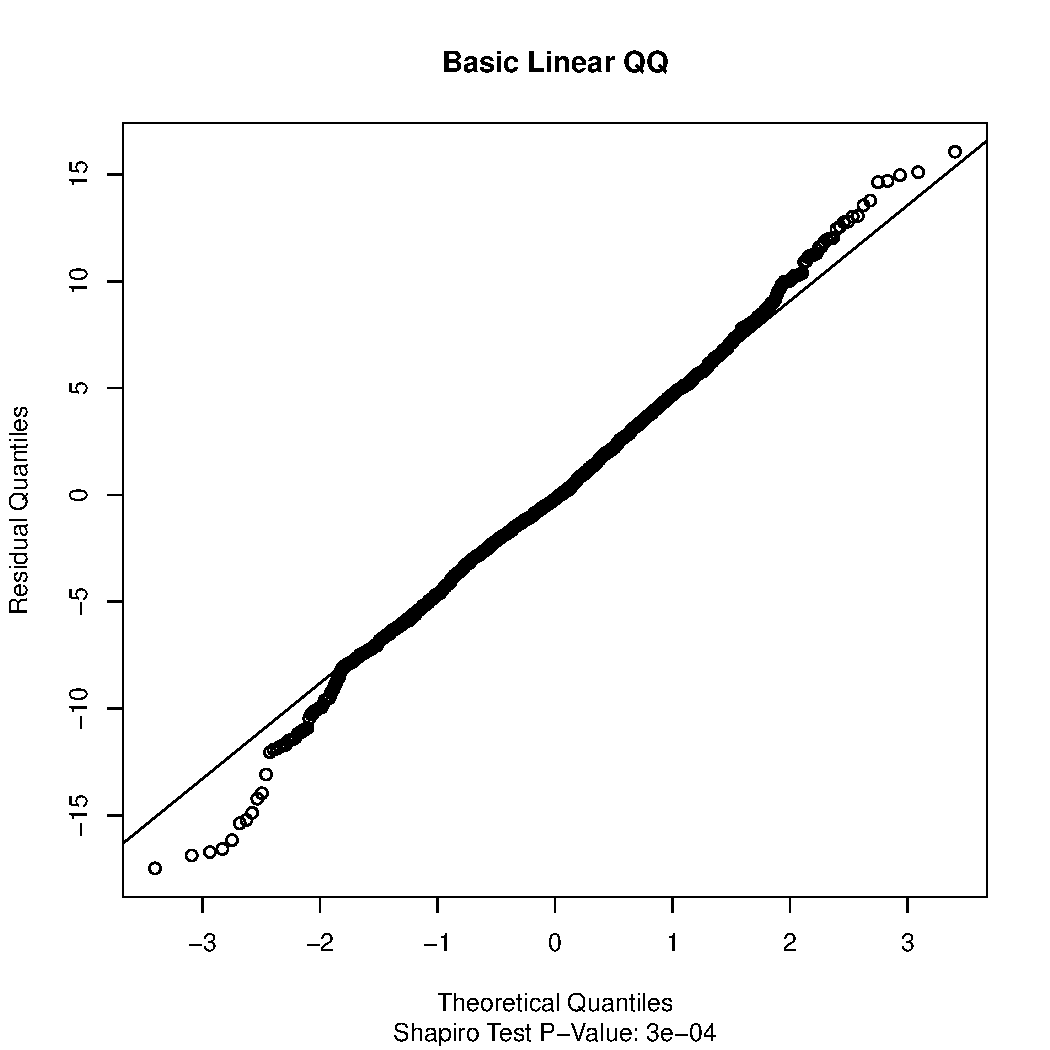
\includegraphics[width=9cm]{final/1a_qq} 
                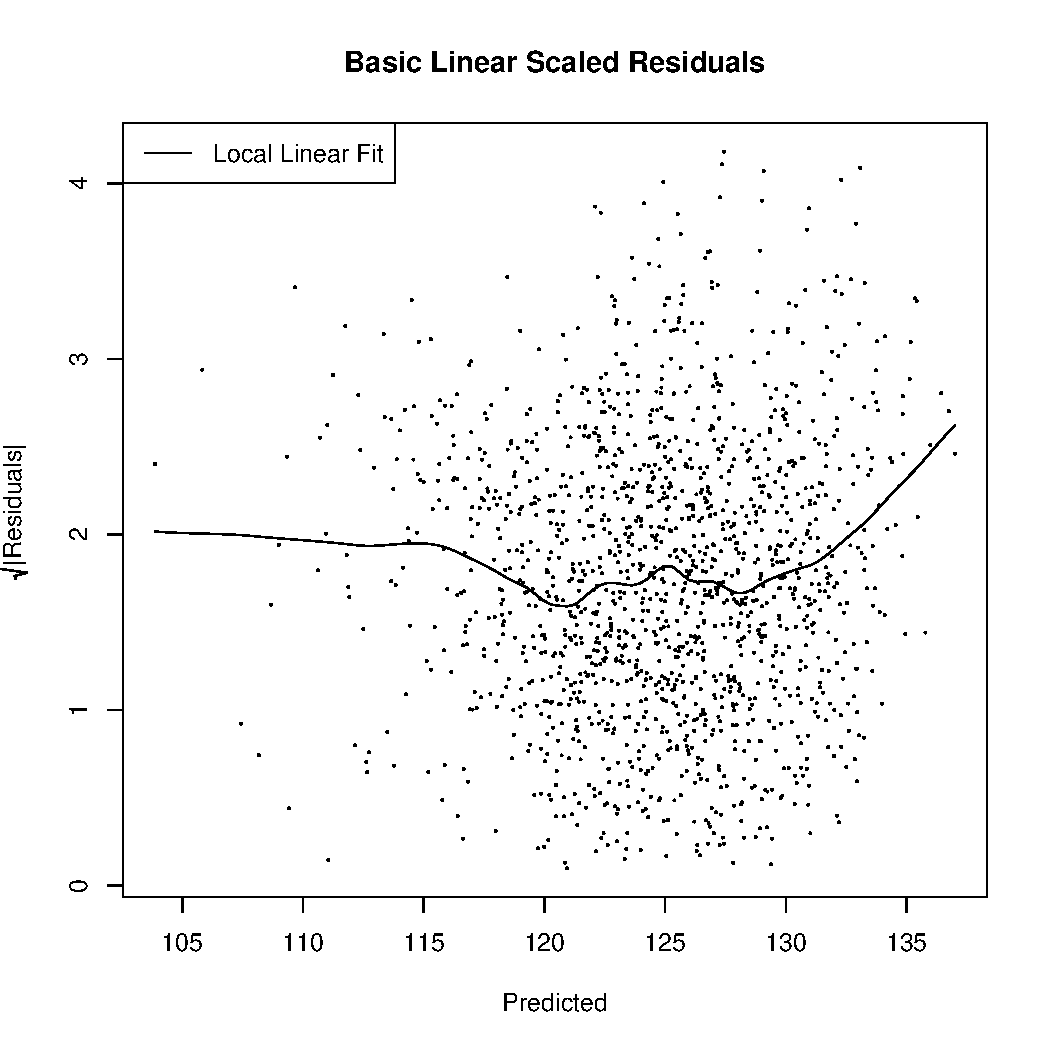
\includegraphics[width=9cm]{final/1a_sqrt_res_plot} \\ 
                In the QQ plot, we see that the distribution of the residuals has much somewhat thicker tails than a normal distribution, though stays pretty close otherwise. The Shapiro-Wilkes test, with a p-value of $.0003$ has us reject normality, but the predictions are still unbiased if the normality assumption doesn't hold, and the deviation from normality is pretty small. The variation in the variance of the residuals doesn't look terrible, but the local linear regression fit seems to show some meaningful variation over the range of predictions. Thus, I ran a new model where, after I scaled the variables so they all go from $0$ to $1$, I transformed the predictors, taking the square root of one minus angle, chord length, and thickness, and the square root of velocity. This resulted in the following model: \\
                \lstinputlisting[firstline=40,lastline=60]{final/1_out.txt}
                Checking the fit again, I see some mild improvement: \\
                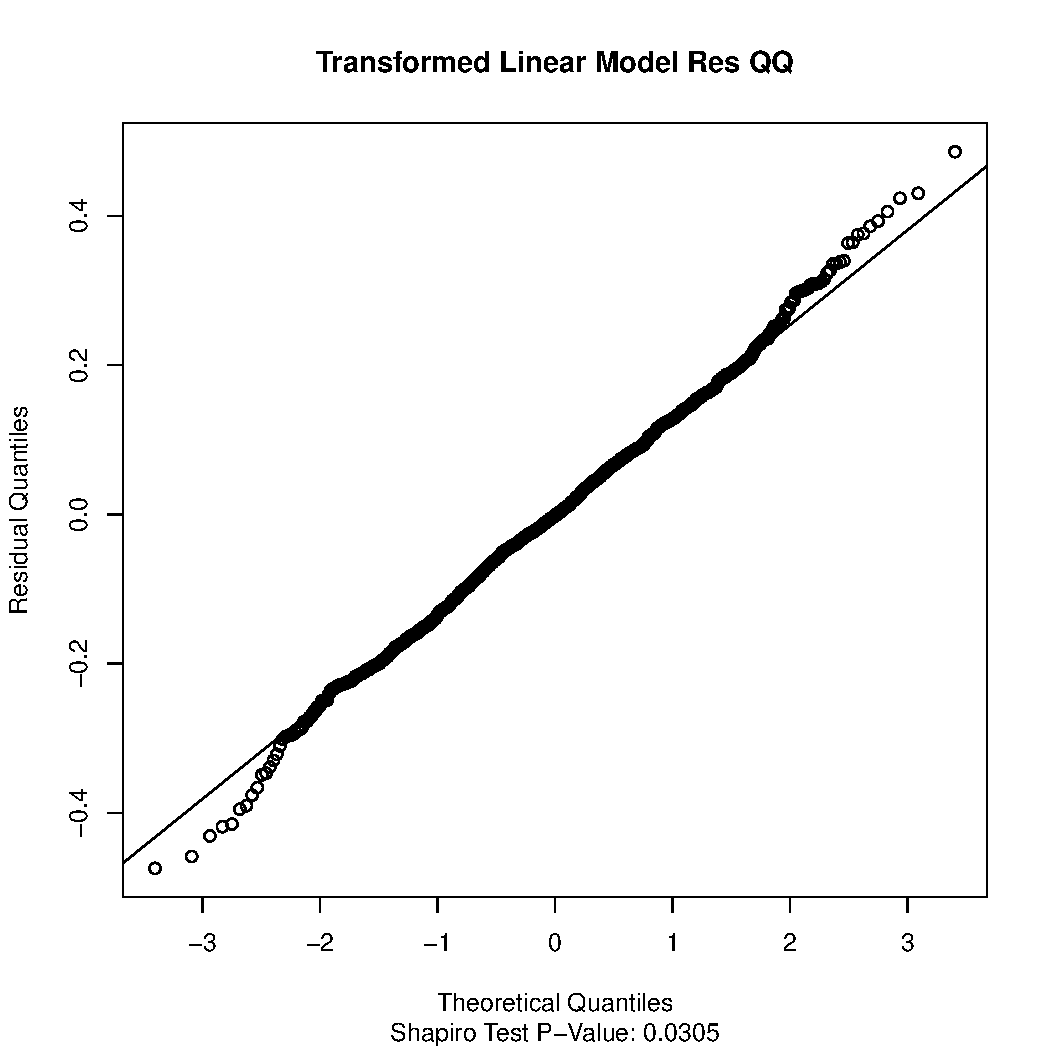
\includegraphics[width=9cm]{final/1a_qq_lm2} 
                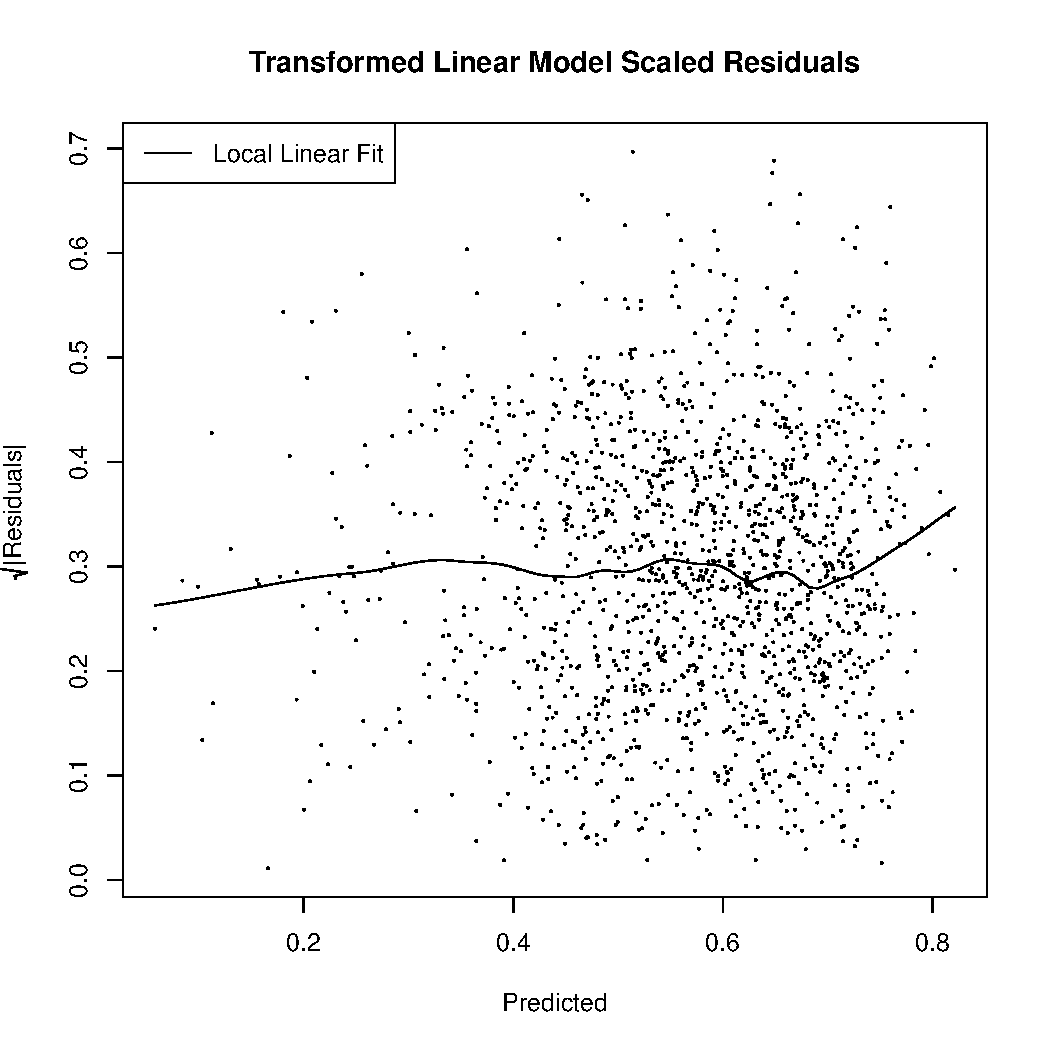
\includegraphics[width=9cm]{final/1a_sqrt_res_plot_lm2} \\ 
                The Residuals are a tad closer to being normally distributed (the lower tail deviates a little less), but more importantly, as one can see from the linear fit, the variance appears to vary much less over the range of predictions, and looks close to being constant, except maybe at the end.
            \item[b)]
                {\bf Summary:} We seem to have some pretty meaningful nonlinearity in the model from part a. To improve upon it, I transform the outcome, pressure, by taking it square root, and replace the terms for frequency, angle, and chord length with a fourth degree polynomial of those three variables together. This reduced the non-linearity and vastly improved the overall fit, as judged by adjusted R-squared. \par
                {\bf Work:} I checked for non-linearity in the model from part a by plotting the residuals by predicted value and a few of the variables (the other two only have a few unique values and looked fine): \\
                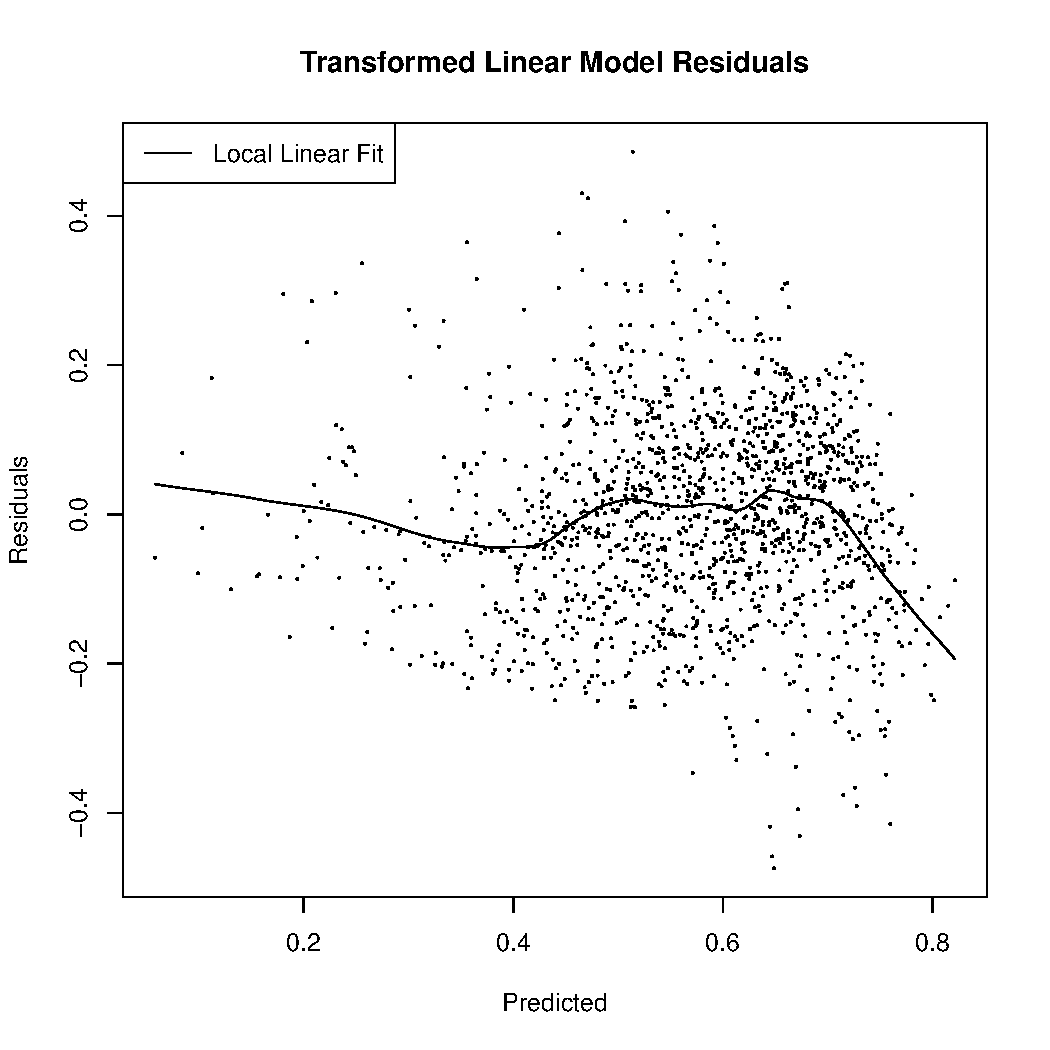
\includegraphics[width=9cm]{final/1b_res_plot_lm2} 
                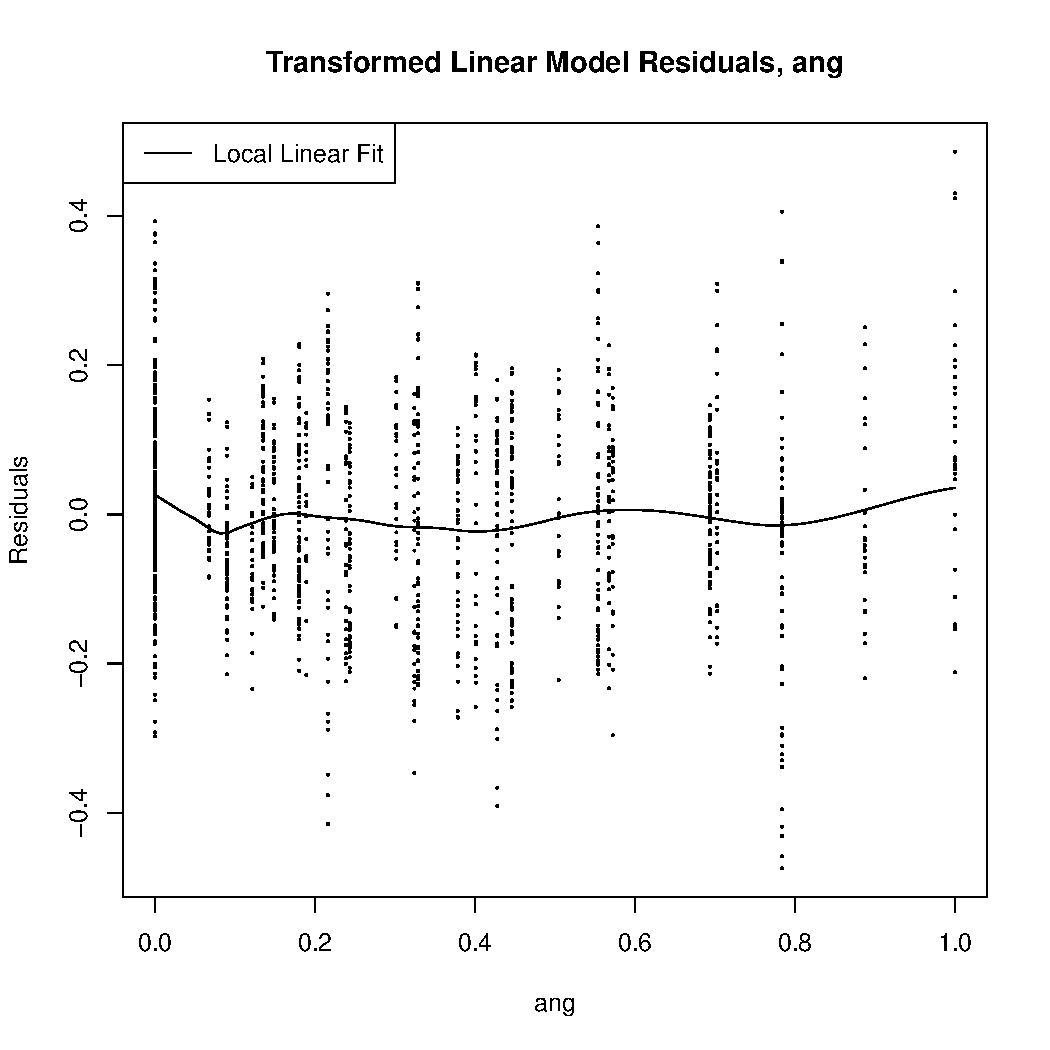
\includegraphics[width=9cm]{final/1b_res_plot_tran_ang} \\ 
                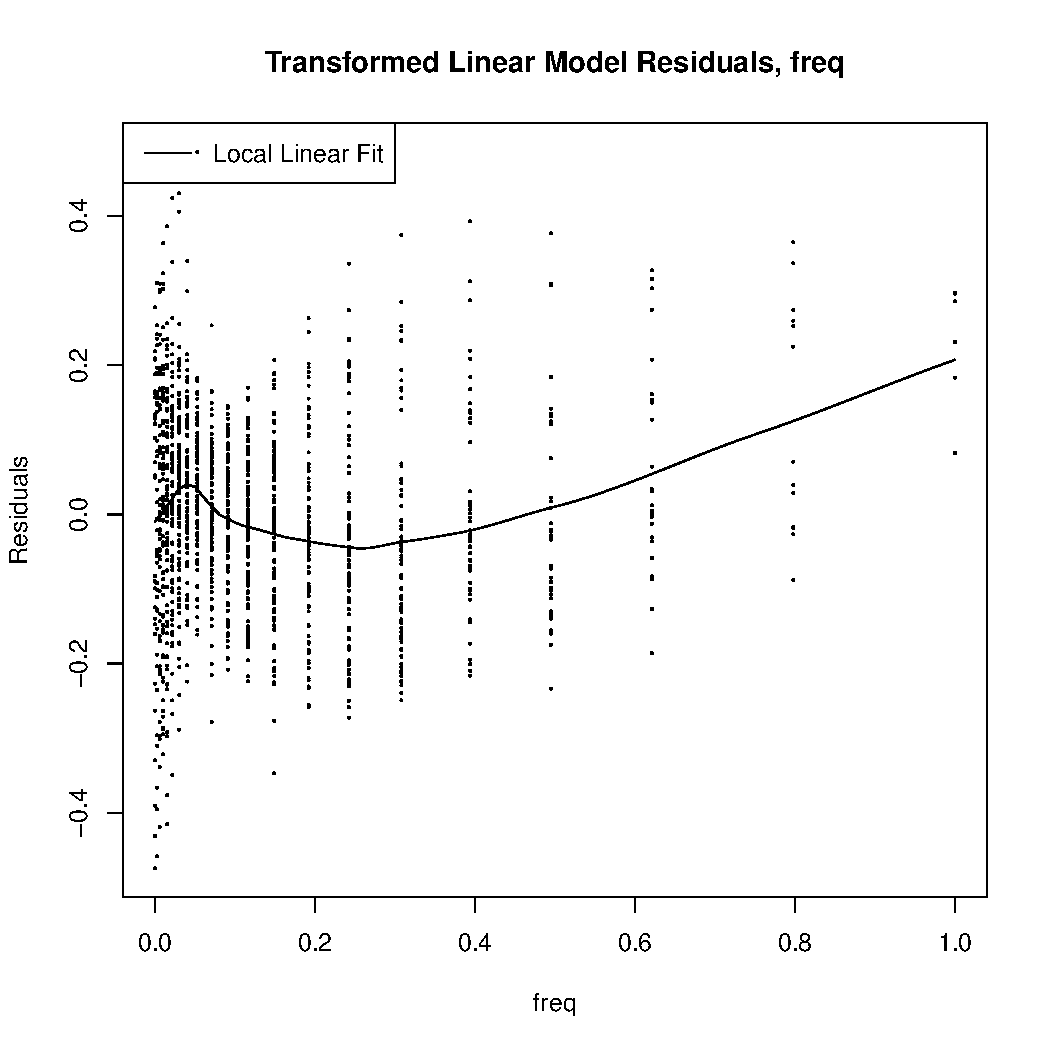
\includegraphics[width=9cm]{final/1b_res_plot_tran_freq}  
                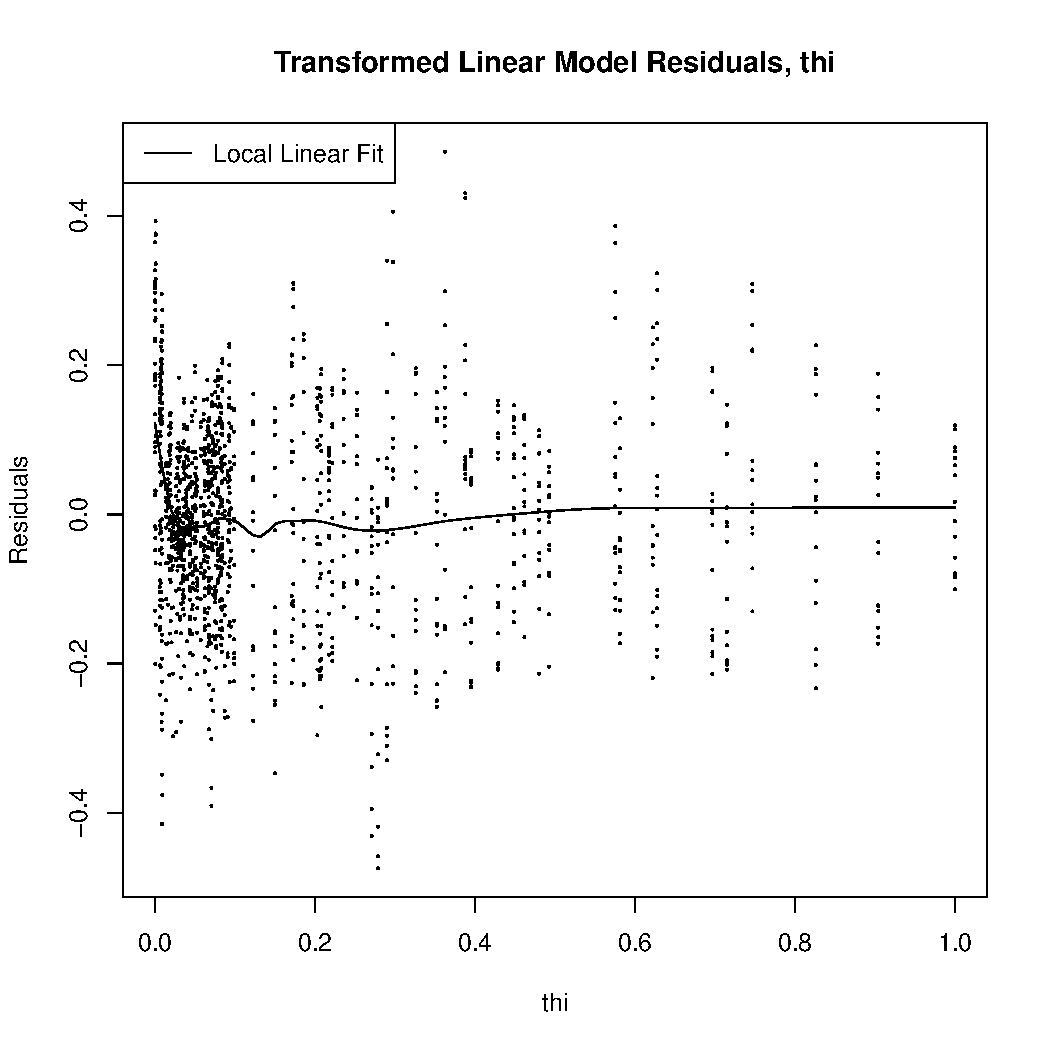
\includegraphics[width=9cm]{final/1b_res_plot_tran_thi} \\ 
                As you can see, the local linear fits pretty strongly show that the residuals don't have a mean of $0$ over the range of predicted values nor range of frequency, even if it looks OK for angle and thickness. I couldn't find any way to remedy this without interactions; I tried a number of models which had every predictor as a factor and some kind of transformation of the outcome, since this would admit every possible transformation of each predictor, but every model still failed to have residuals with mean $0$ over the range of predicted values. Thus, I introduced a set of orthogonal polynomials of degree up to 4 in terms of frequency, angle, and chord length together, as well as took the square root of pressure. This is the resulting model summary: \\ 
                \lstinputlisting[firstline=76,lastline=127]{final/1_out.txt}
                There are a lot of variables added, but not that many considering the size of the data set, and we see a big overall improvement in fit, as shown by the adjusted $R^2$ increasing to $.813$ from $.477$. Looking at plots of the residuals, we also seem to have mostly mitigated the issues with nonlinearity: \\
                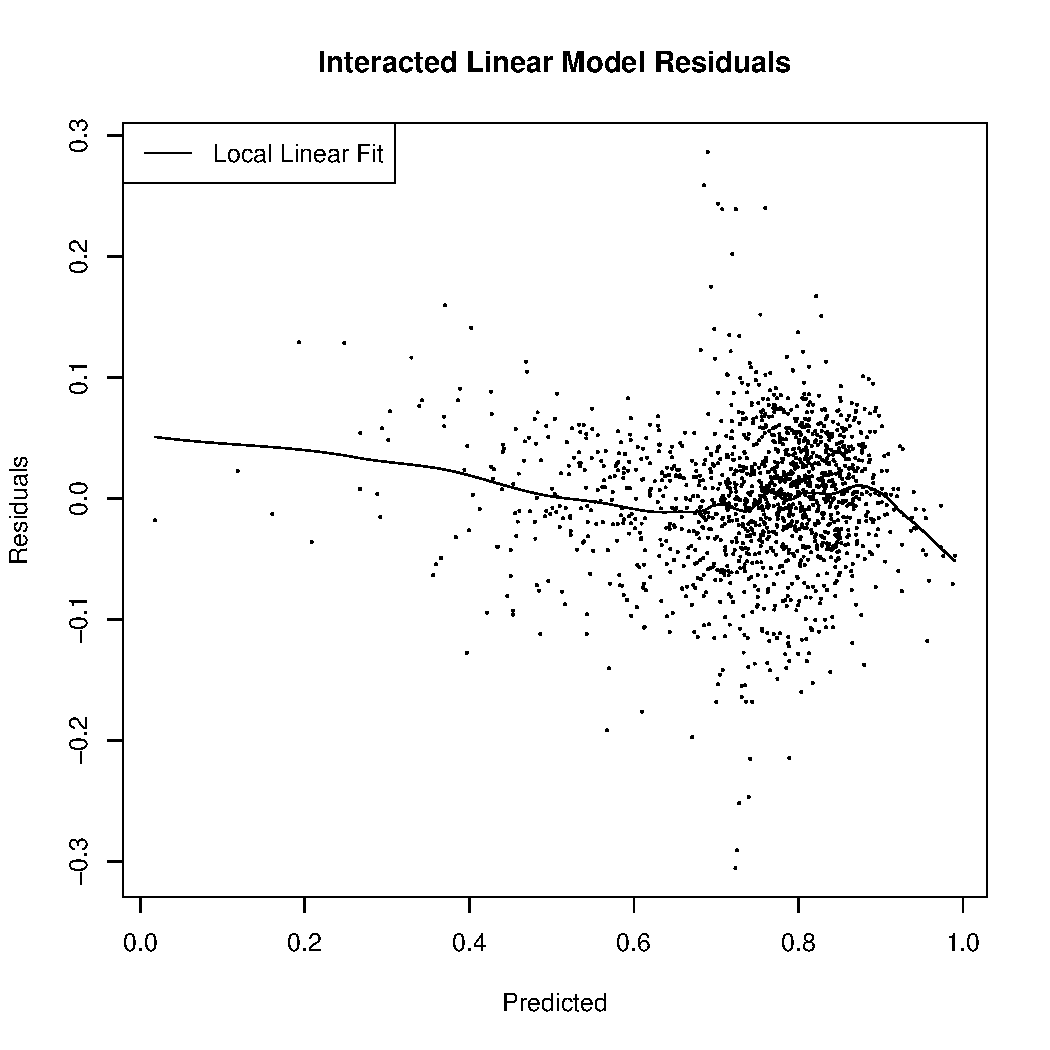
\includegraphics[width=9cm]{final/1b_res_plot_int} 
                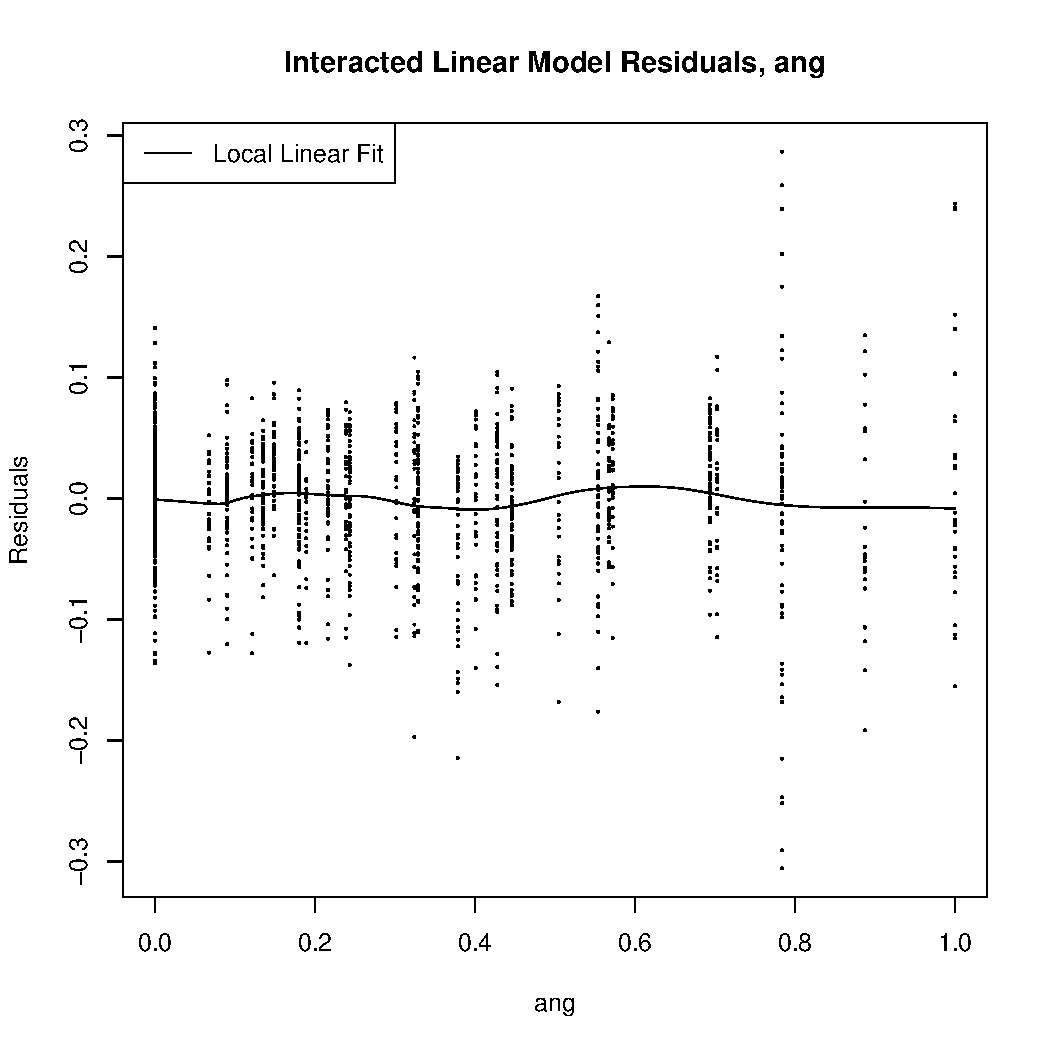
\includegraphics[width=9cm]{final/1b_res_plot_int_ang} \\ 
                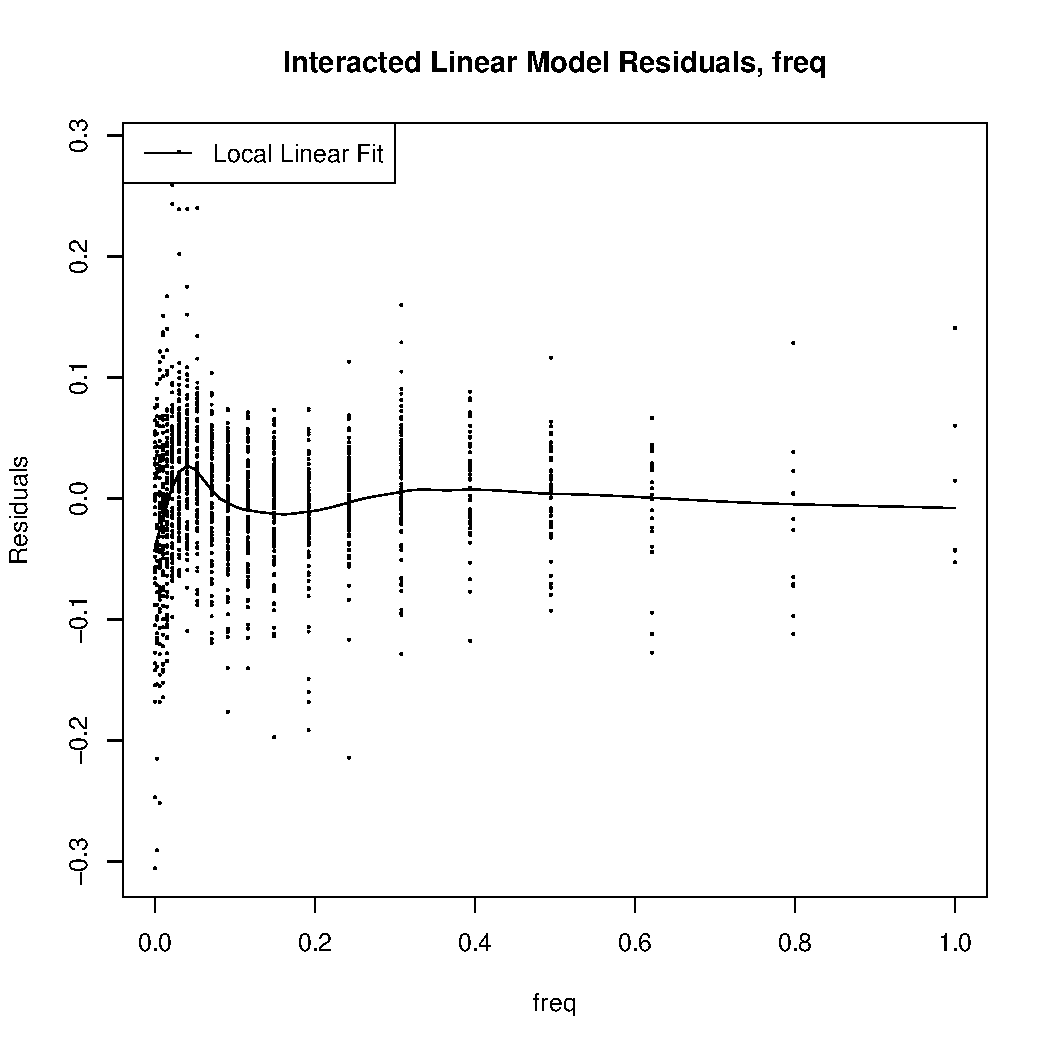
\includegraphics[width=9cm]{final/1b_res_plot_int_freq}  
                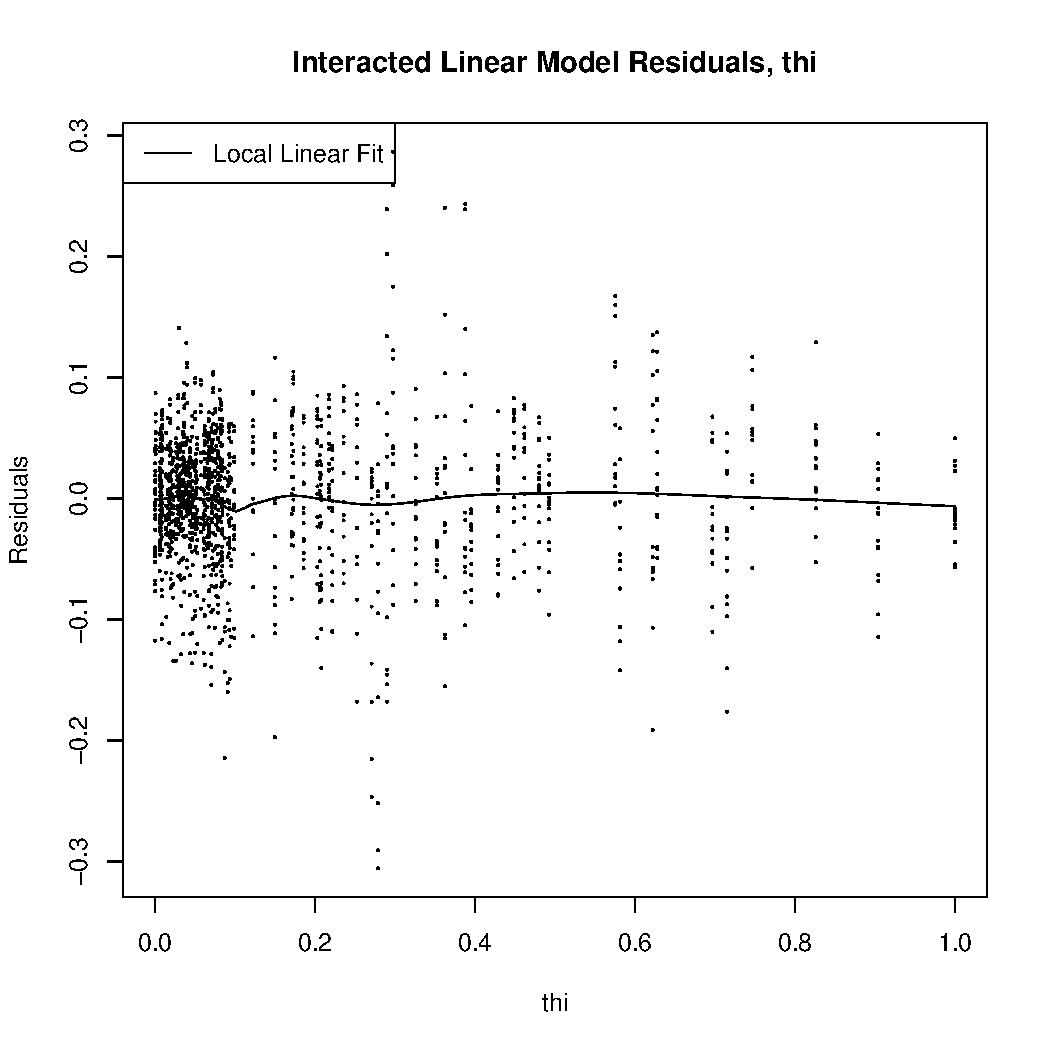
\includegraphics[width=9cm]{final/1b_res_plot_int_thi} \\ 
                While there is still some nonlinearity, the mean is consistently right around $0$, except in a few spots with sparse data. We do seem to have meaningful non-zero means at lower frequencies, and at the higher end of the predicted values, but these biases are small, and much better than with the previous model. Double checking the variance, we seem to still have close to constant variance, with possibly a little less consistency than we had before: \\
                \begin{center}
                    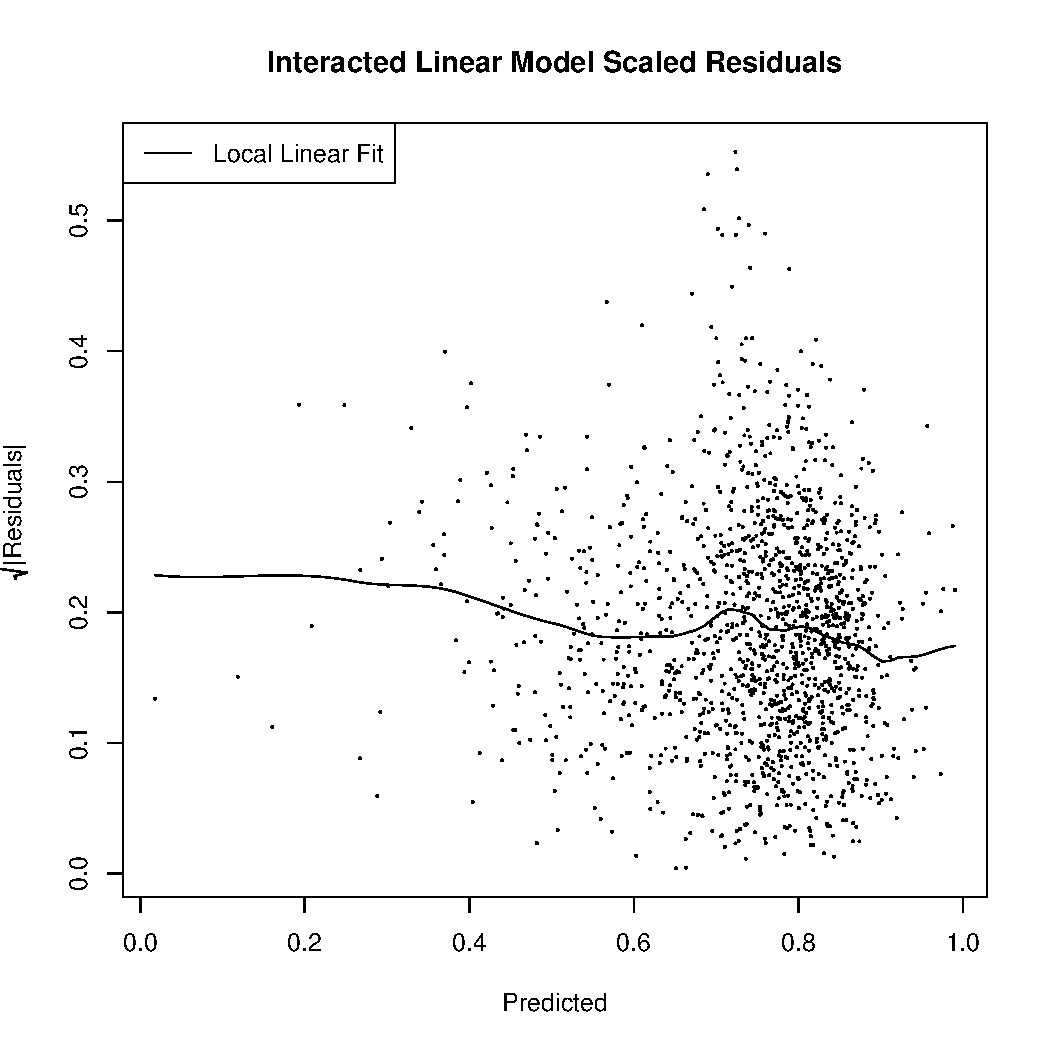
\includegraphics[width=9cm]{final/1b_sqrt_res_plot_int} 
                \end{center}
            \item[c)]
                Of these two, each has its own advantages. The model from part a has the advantage of simplicity,, while only mildly violating the linear model assumptions, making it suitable for explanation. The confidence intervals obviously won't be perfect, since the predictions are biased and the normality assumption doesn't hold. However, the confidence level is high enough that we can still fairly safely say that the predicted positive or negative correlations between the predictors and outcome hold true, and the estimates of how much this is by serves a sufficient ballpark guess. On the other hand, the model from b does seem to fulfill the assumptions of a linear regression model mostly (except possibly normality) and has high $R^2$, so it is good for prediction, even if the confidence intervals of the prediction might be slightly off. It is just convoluted enough that it is hard to interpret what effect angle, frequency, and chord length have on pressure without making a visual, since there are no single coefficients on these predictors.. 
            \item[d)]
                Fitting a tree model, I pruned the tree at a complexity parameter of $3.31*10^{-6}$. Any split which didn't decrease total $R^2$ by at least that much was discarded. This was chosen because it was the points at which $10$ fold cross validation estimated there would be the lowest error. This gave a tree with $1121$ splits for $1502$ data points, which seems like a lot, but when one calculates the adjusted $R^2$, the result is still an impressive $.999$, having reduced the $RSS$ to $27.467$ from it original value of $71480.51$. Between this and the cross validation, we are reasonably assured that this is not an over fit. We can look at the distribution of the residuals:\\
                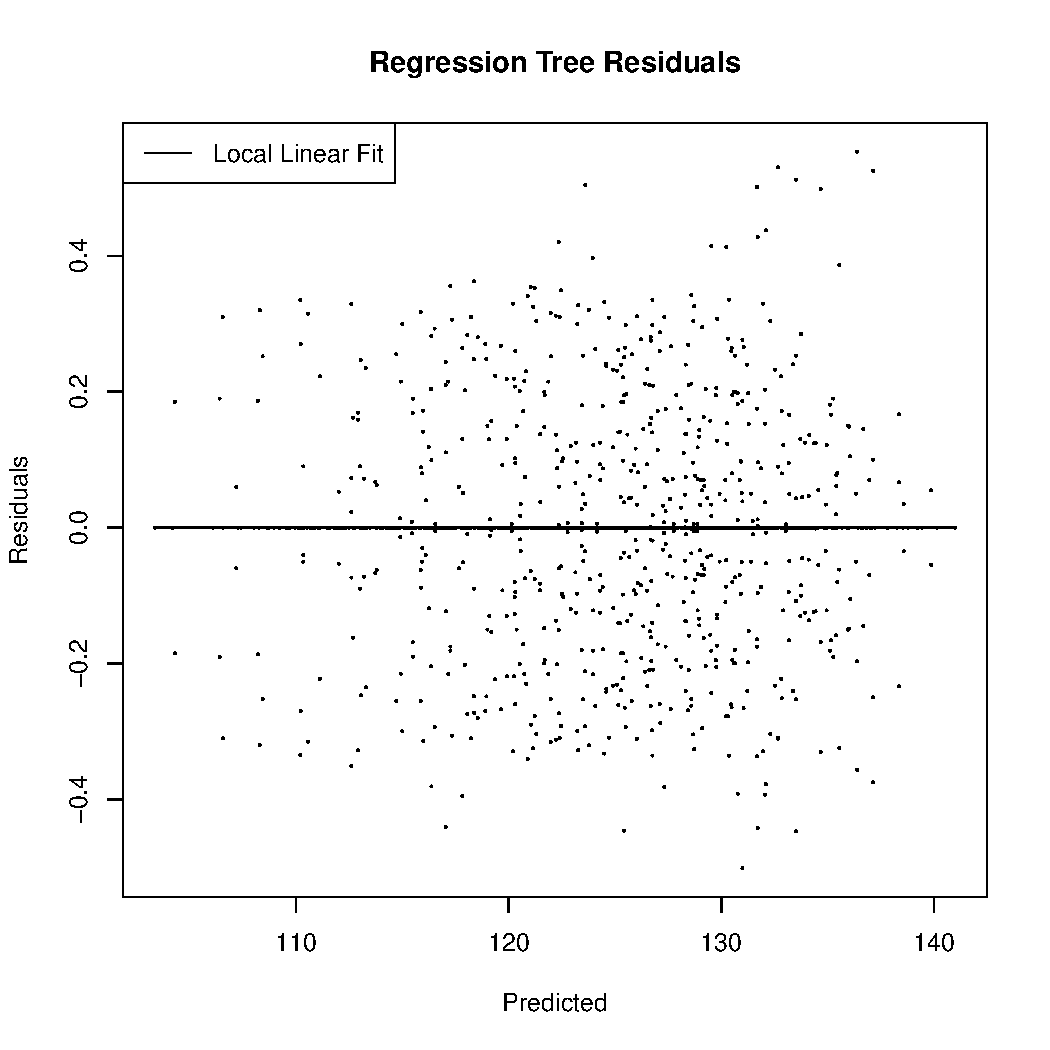
\includegraphics[width=9cm]{final/1d_res_plot_tree} 
                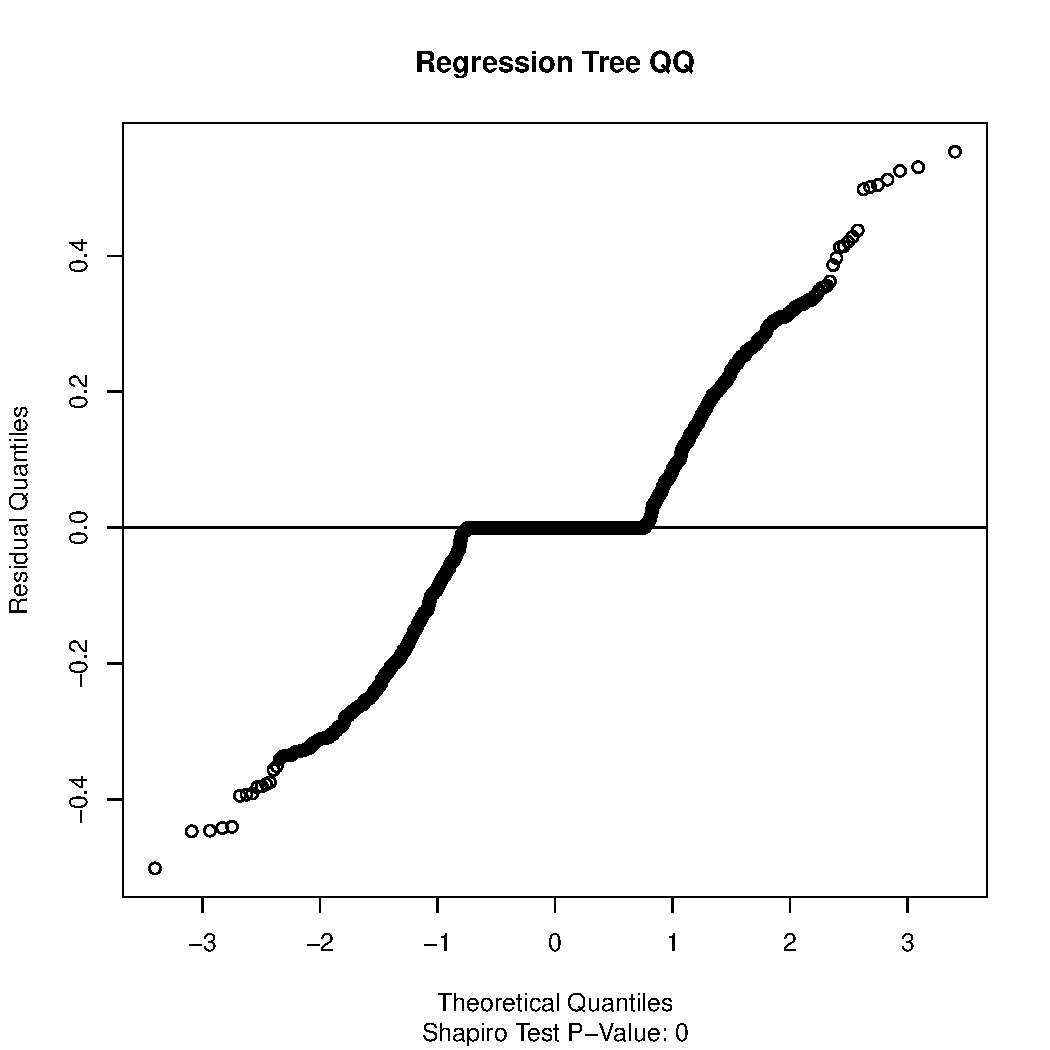
\includegraphics[width=9cm]{final/1d_qq_tree} \\
                As we would expect, by construction, the residuals definitely have mean $0$, with a large number of them, in fact, being $0$. Additionally, the residuals are no where close to normally distributed, but this is to be expected with so many of them already at $0$.
            \item[e)]
                As we we have seen here, in data that doesn't naturally fit the assumptions necessary for linear regression, its hard to transform it to the point where all the assumptions hold well. One can add an arbitrary amount of flexibility to a linear model to make it work, through splines, polynomials, other spanning function bases, and the like, but this has to be done manually. By the point enough flexibility has been added, often there is no easy interpretation of coefficients. Here in lies the advantage of a tree model; it has arbitrary amounts of flexibility built in by default, making it appropriate and easier for prediction with this kind of messy data. If you happen to stumble on a data set that actually has a linear relationship between two variables though, a tree model will never predict quite as well nor be as interpretable as the linear regression.

        \end{itemize}

    \item[2.]
        \begin{itemize}
            \item[a)]
                This is the summary from the linear model: \\ 
                \lstinputlisting[firstline=3,lastline=21]{final/2_out.txt} 
            
                \begin{itemize}
                    \item[i.]
                        This residuals are pretty close to normal for the most part, but is different enough that we can say with a high degree of certainty that weren't actually drawn from normal distribution. Looking at the QQ plot of the residuals, the quantiles of residuals line up pretty well with normal quantiles except at the lower tail (perfect correspondence is falling along the line). At the lower tail though, there is immense deviation from the normal quantiles. With such a huge data set, such a large deviation for so many points is extremely unlikely. The end result is that we can expect the estimated confidence intervals (from the normal assumption) will be somewhat off.
                        \begin{center}
                            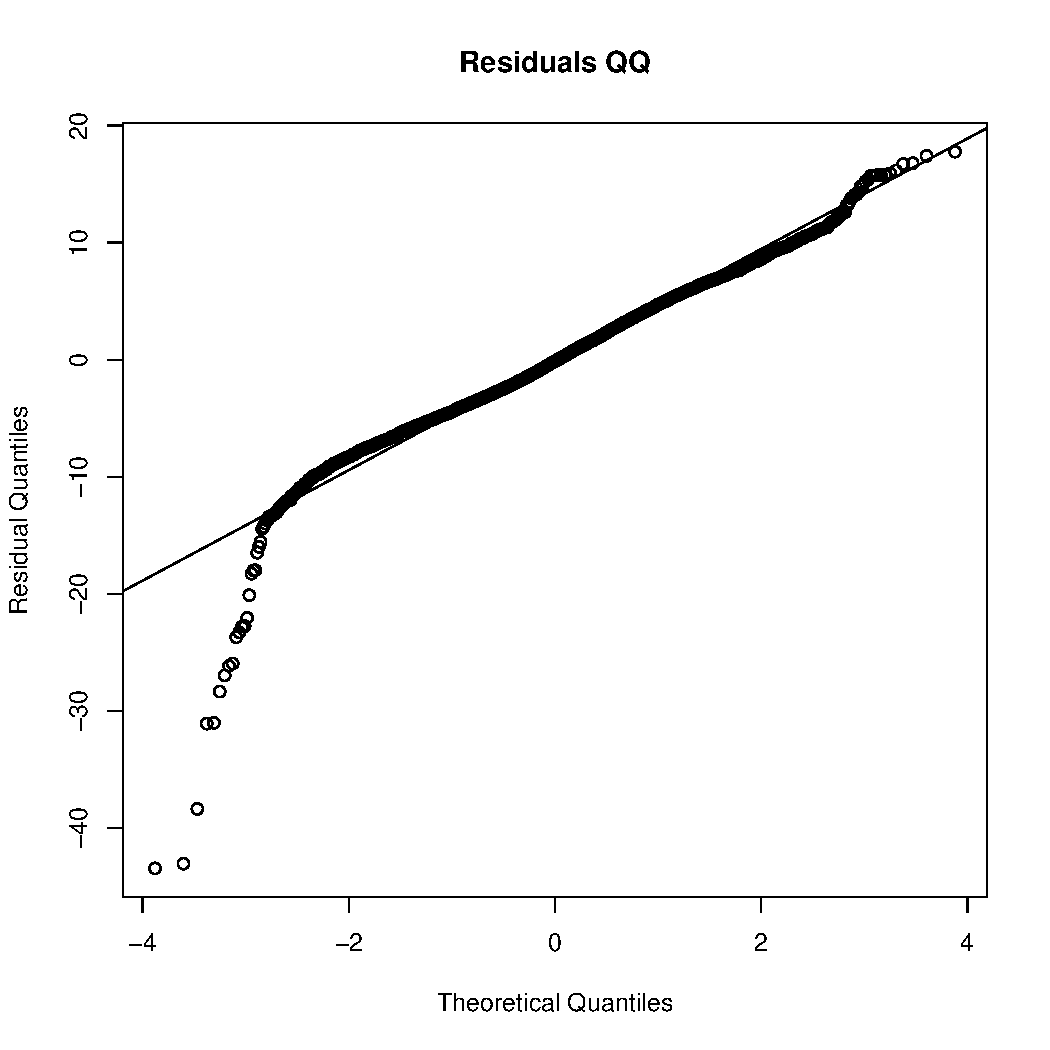
\includegraphics[width=9cm]{final/2ai_qq} 
                        \end{center}

                    \item[ii.]
                        There are unquestionably pretty significant outliers. We can see this by looking at the Cook distance and the studentized residuals. I have plotted a quantile plot of the studentized residuals below. The Bonferroni Critical value for the absolute value of studentized residuals at an alpha of $.05$, which is the \(\frac{1-.05/2}{n}\) quantile of a t distribution with $n-p$ degrees of freedom, is $4.5581$. By comparison, looking at the plot, we can see that there are a number of studentized residuals with an absolute value greater than $4.5581$, going as high as $9.5778$. Since this critical value is conservative, we definitely have a number of outliers.
                        \begin{center}
                            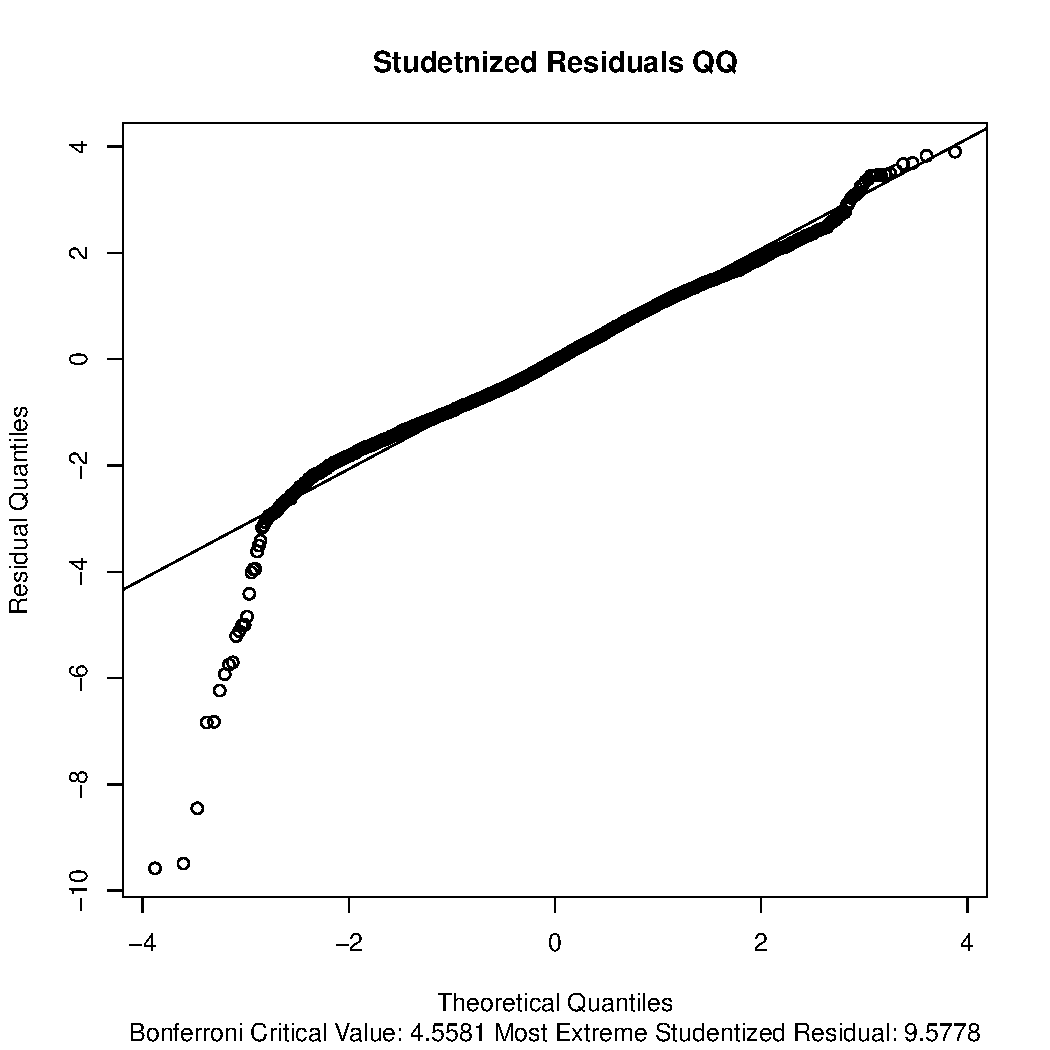
\includegraphics[width=9cm]{final/2aii_stud_qq} 
                        \end{center}
                        Looking at this another way, we consider the Cook distances, plotted against the half-normal quantiles. We certainly seem to have some Cook distances which stand out; this further supports the notion we're looking at outliers.
                        \begin{center}
                            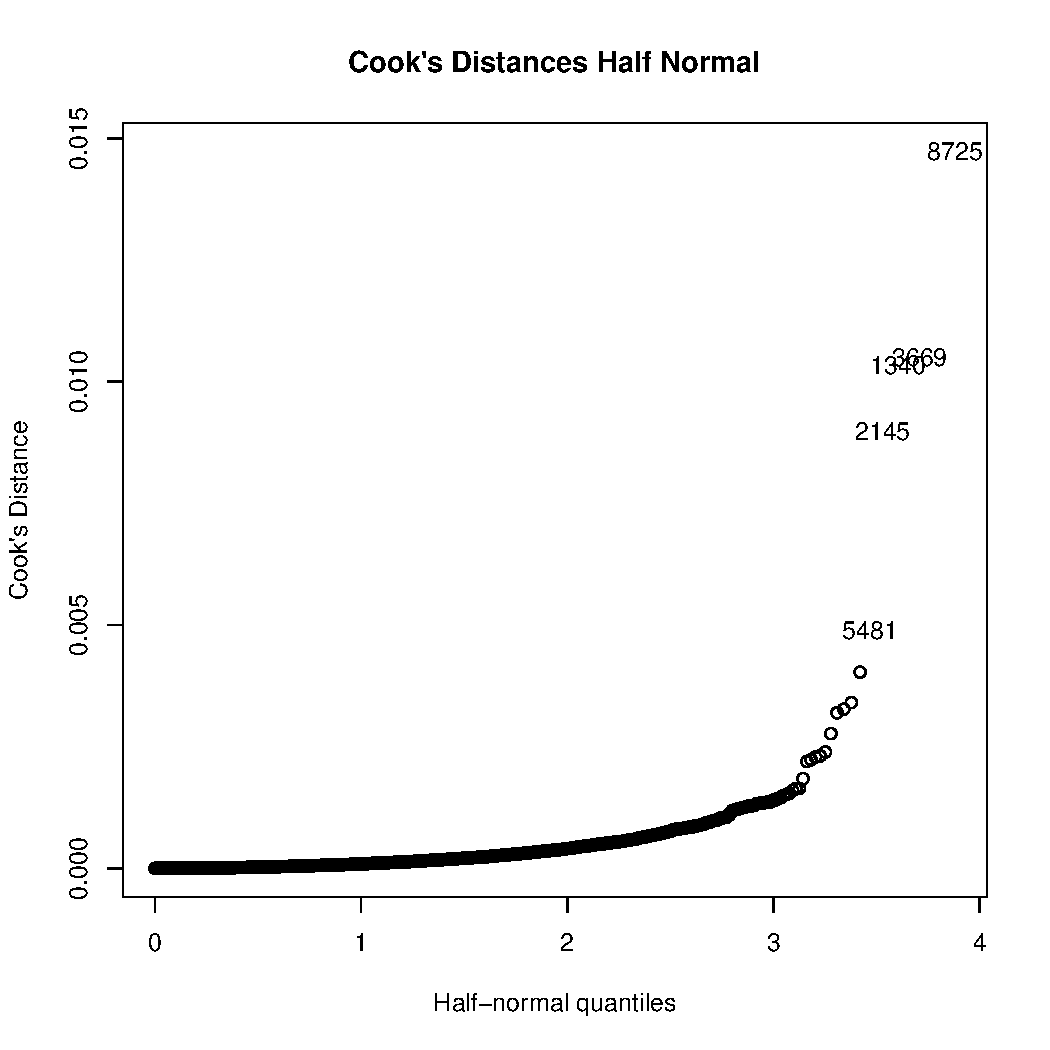
\includegraphics[width=9cm]{final/2aii_cook} 
                        \end{center}
                    \item[iii.]
                        The linearity assumption seems to hold up for the most part. The first check is that the residuals really do have mean $0$ throughout the range of predictions. Plotting the residuals against the predicted values and fitting a flexible kernel regression model, we do seem to have very close to mean $0$, except at the lowest end of the predicted range; the local regression is very close to $0$ everywhere else.               
                        \begin{center}
                            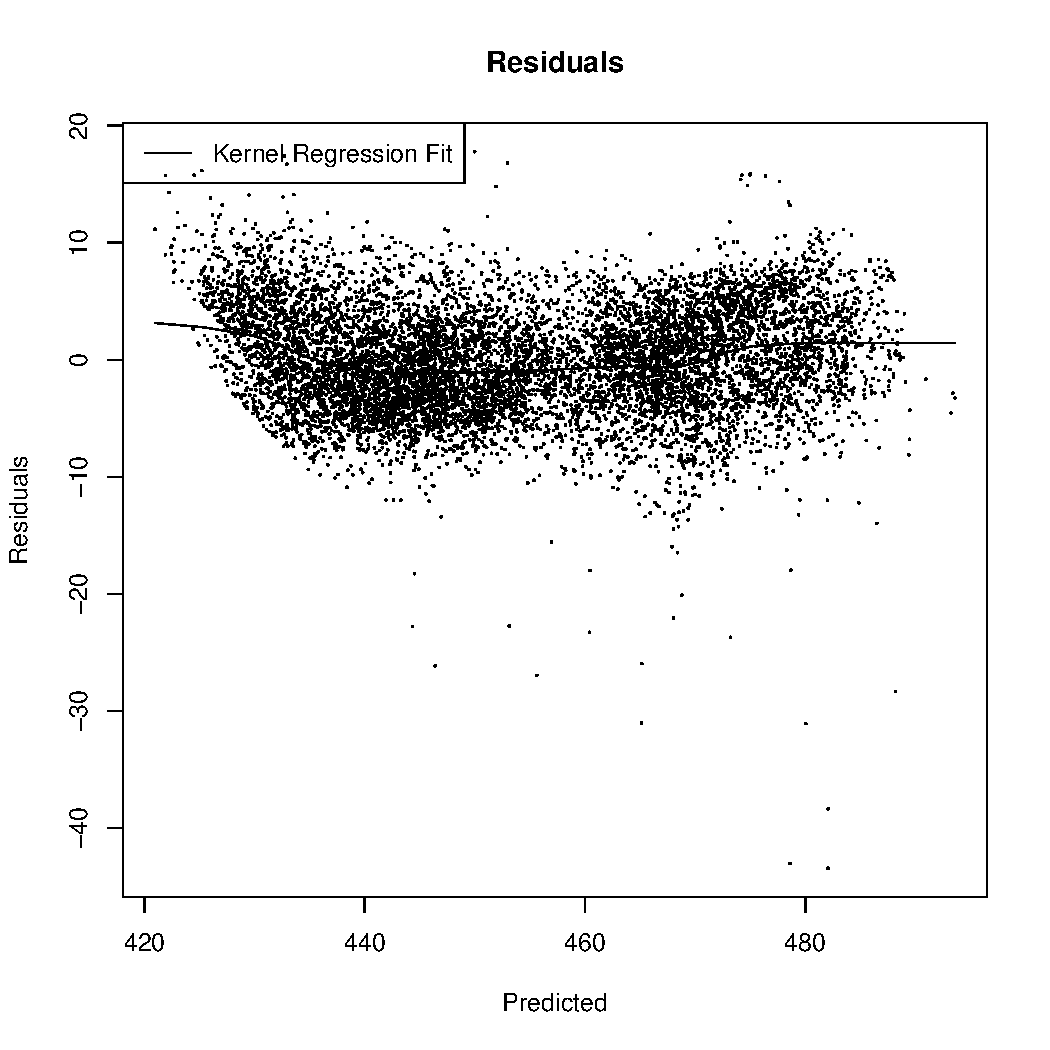
\includegraphics[width=9cm]{final/2aiii_res_plot} 
                        \end{center}
                        Additionally, checking the partial residual plot of each variable in turn, all of them the linear fits seem to be extremely good. If there isn't a linear relationship between one of the variables and the outcome, the difference isn't much. \\
                        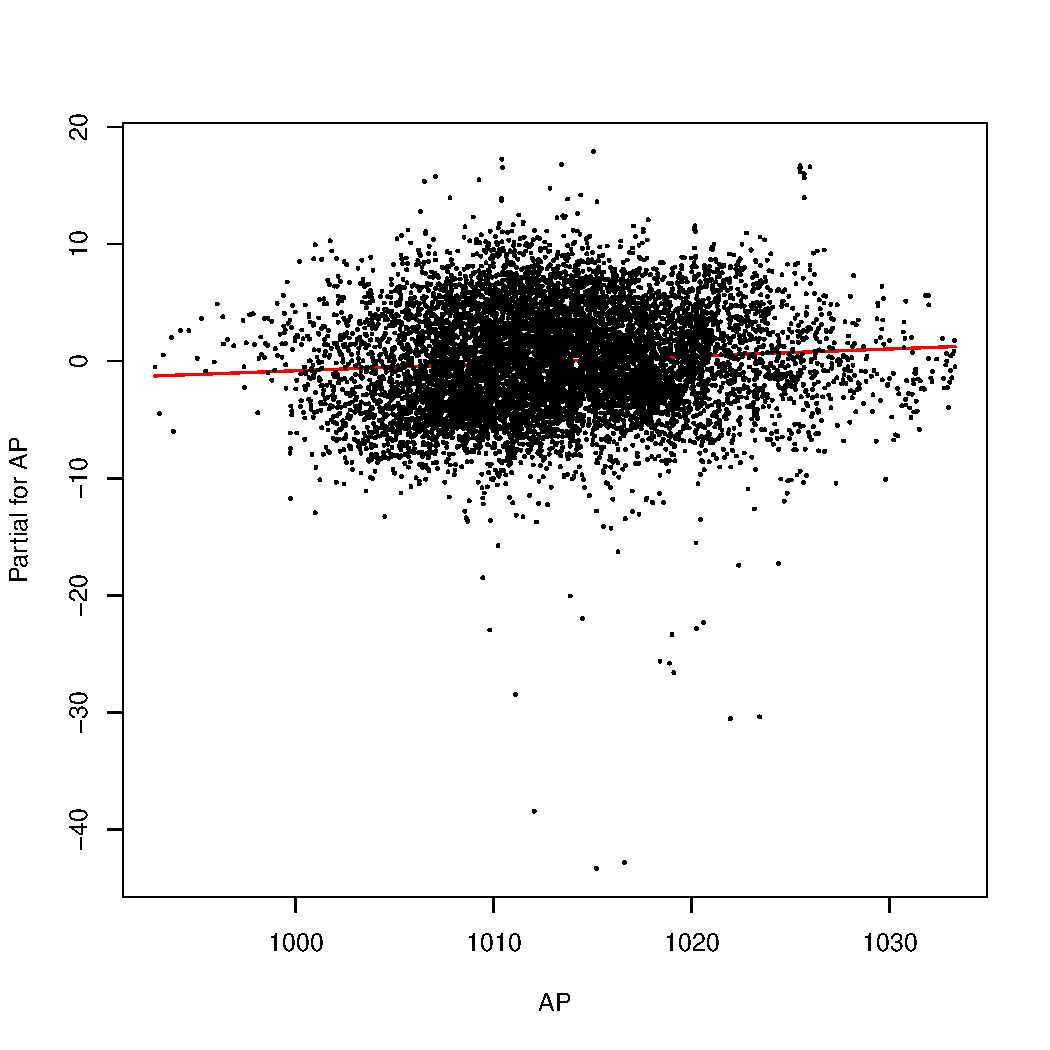
\includegraphics[width=9cm]{final/2aiii_pr_AP} 
                        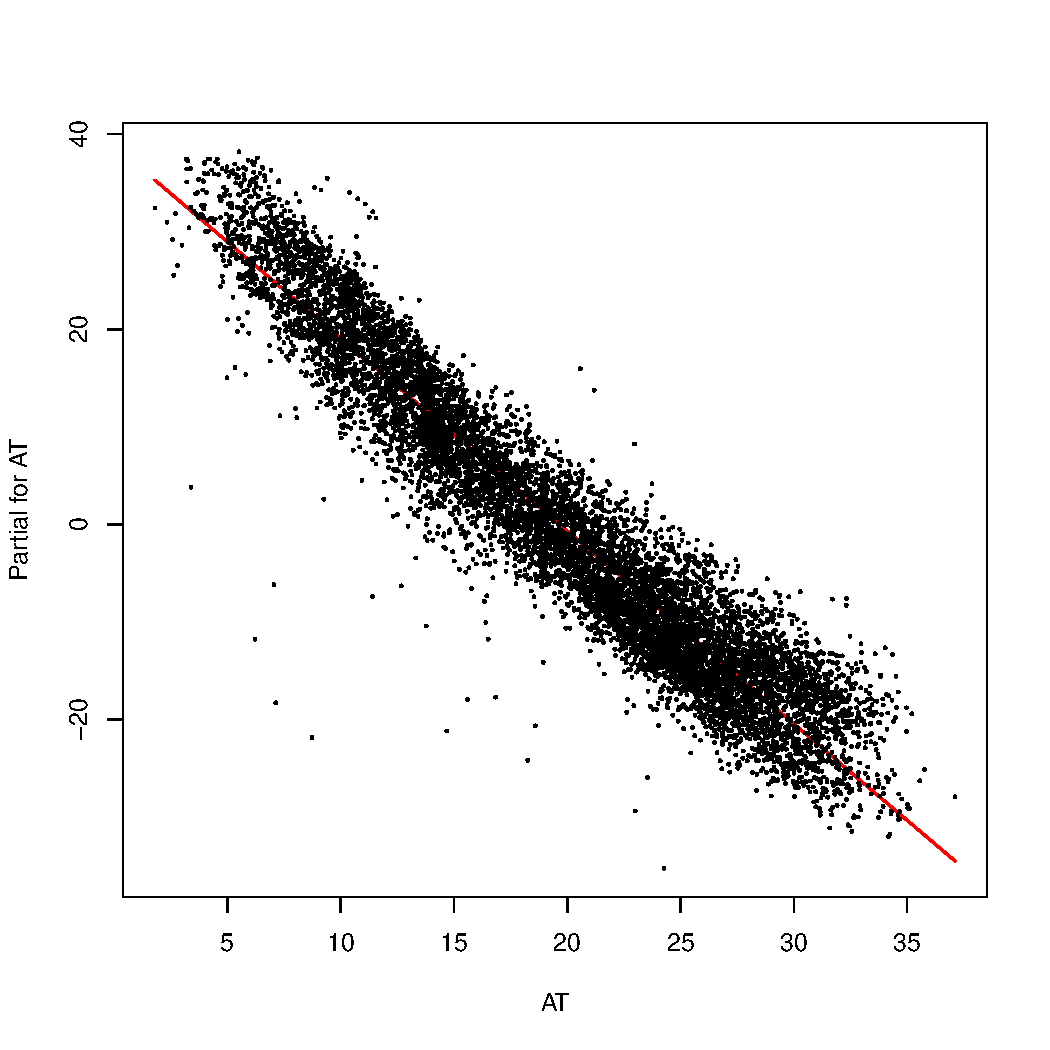
\includegraphics[width=9cm]{final/2aiii_pr_AT} \\ 
                        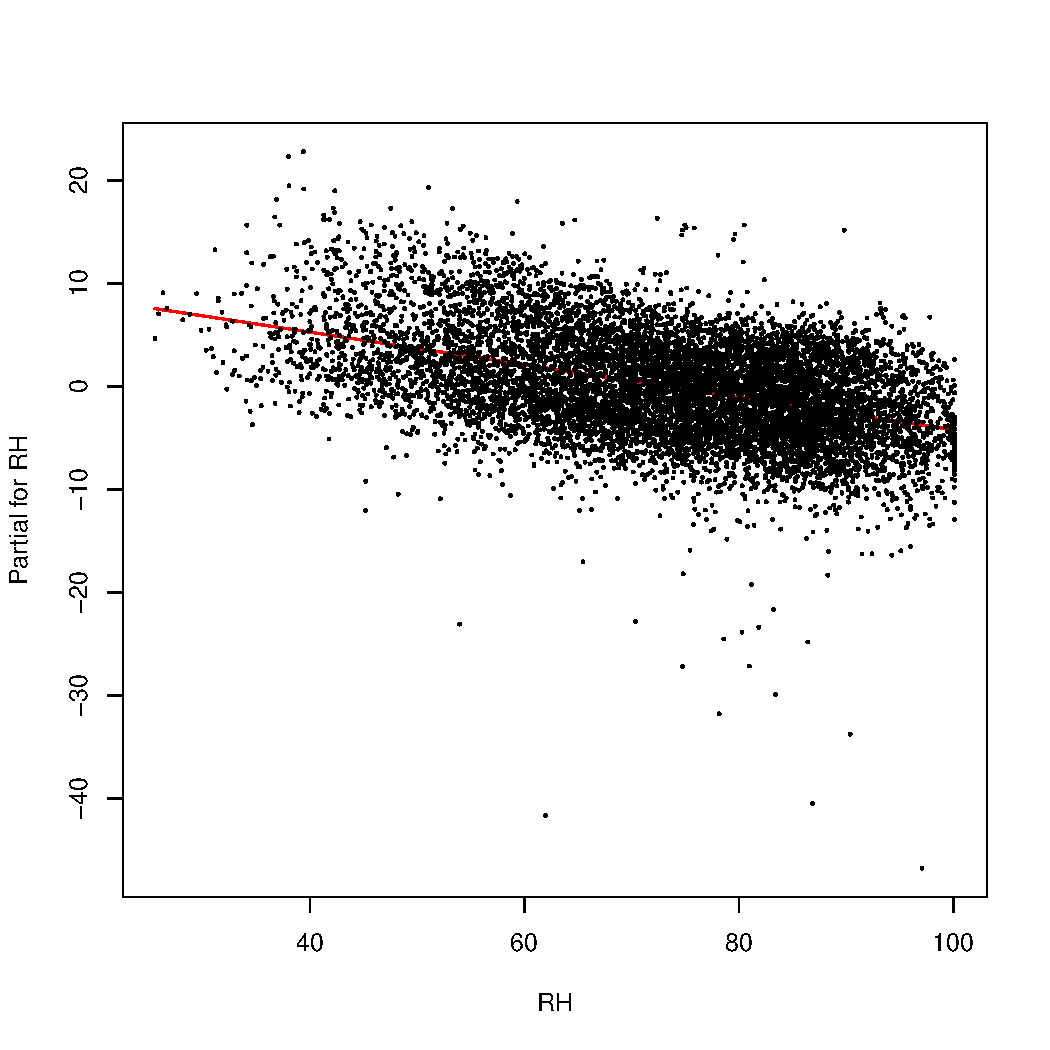
\includegraphics[width=9cm]{final/2aiii_pr_RH} 
                        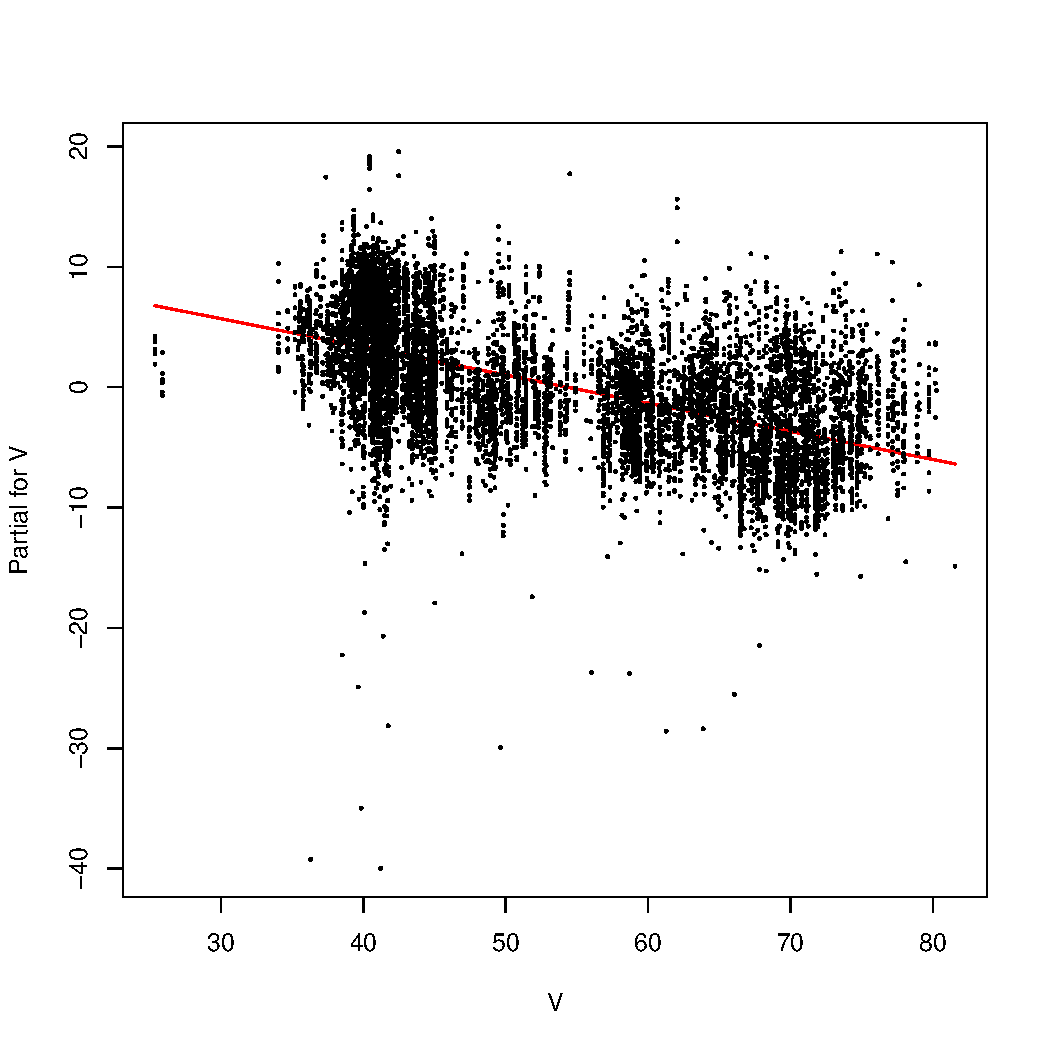
\includegraphics[width=9cm]{final/2aiii_pr_V} \\ 
                \end{itemize}
            \item[b)]
                For both of these statistics, I used a parametric bootstrap methodology to come up with critical values. For each boot, I drew a new set of outcomes $Y^*$, each one drawn from a normal distribution whose mean was the prediction from the original linear model for the given observation, and whose variance was the estimated variance from the original linear model. Using $Y^*$ and the original $X$, I fit a new linear model, and then calculated the statistic (Cook Distance or absolute studetnized residual) from this model for all the observations, keeping the $q$ largest values. After this, the critical value for the $q$th largest value at a p-value of $alpha$ is the $1-\alpha$ percentile of the $q$th largest values from all the boots. In other words, it was chosen so it is larger than $q$th largest value from exactly $\alpha$ of the boots. 
                \begin{itemize}
                    \item[i.]
                        {\bf Summary:} Using the method described above, run for 2000 total boots, I generated critical values for the $1$st through $10$th largest Cook Distances. We reject the ten largest cook distances as outliers, since they fall above these values. \par
                        {\bf Work:}I have plotted the critical values less than $.1$ below. Obviously the critical values should asymptotically approach infinity as they go to $0$. This is only a finite simulation though, so little should be read into the estimates extremely close to $0$.
                        \begin{center}
                            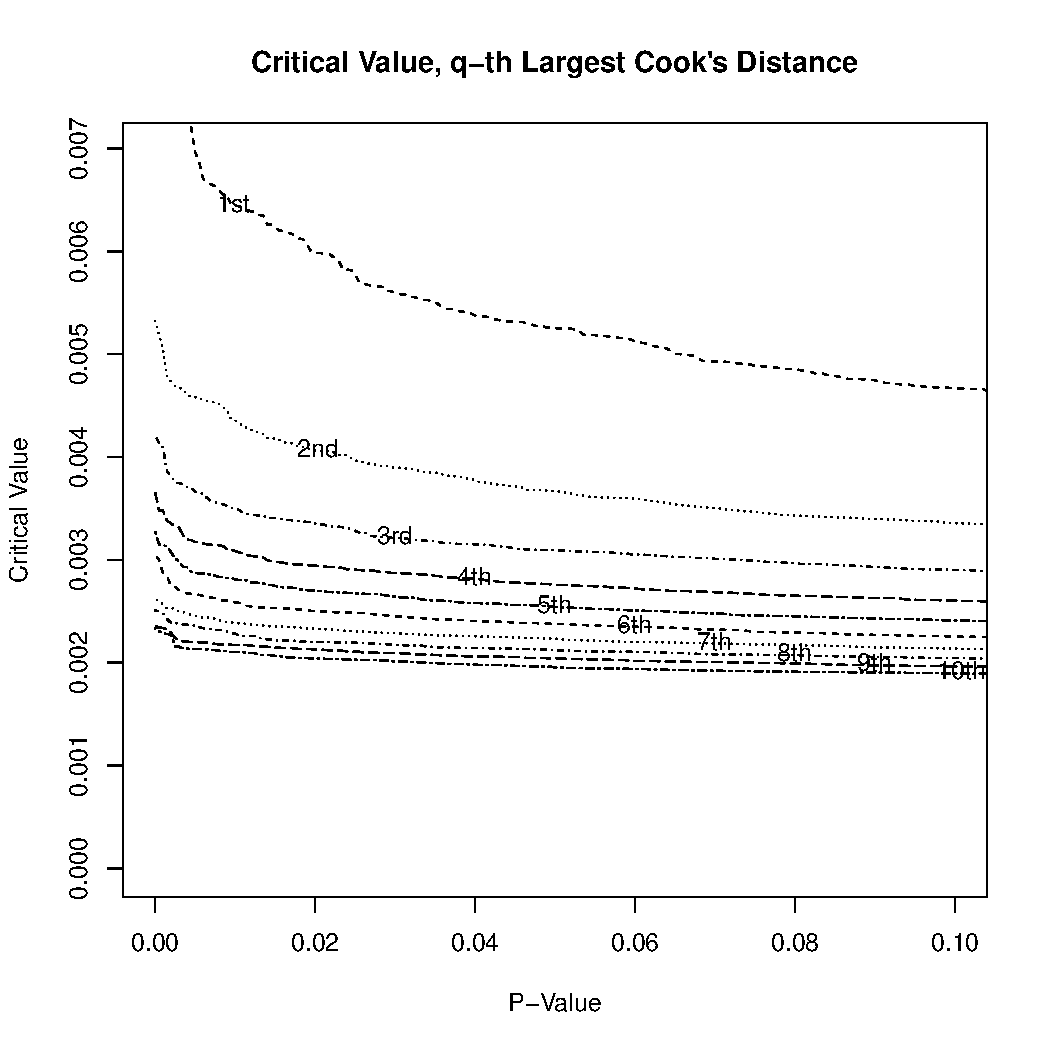
\includegraphics[width=12cm]{final/2bi_plot} 
                        \end{center}
                        Comparing the $1$st-$10$th largest Cook Distances from the original model:\\ 
                        \lstinputlisting[firstline=24,lastline=25]{final/2_out.txt} 
                        To the respective critical values at p-values of $.01$, $.05$, and $.1$: \\
                        \lstinputlisting[firstline=27,lastline=30]{final/2_out.txt} 
                        We see that they all fall outside of the critical values for each confidence level, so we would reject them all as outliers for each confidence level. \\
                        {\bf My R Code:}
                        \lstinputlisting[firstline=191,lastline=214,breaklines=true]{final.R} 

                    \item[ii.]
                        {\bf Summary:} Using the method described above, once again for 2000 total boots, but this time for studentized residuals, I have once generated the critical values. We again reject all $10$ largest studentized residuals as outliers, since they fall outside these values. \par
                        {\bf Work:} The critical values are plotted below. The same issue for critical values extremely close to 0 exists.
                        \begin{center}
                            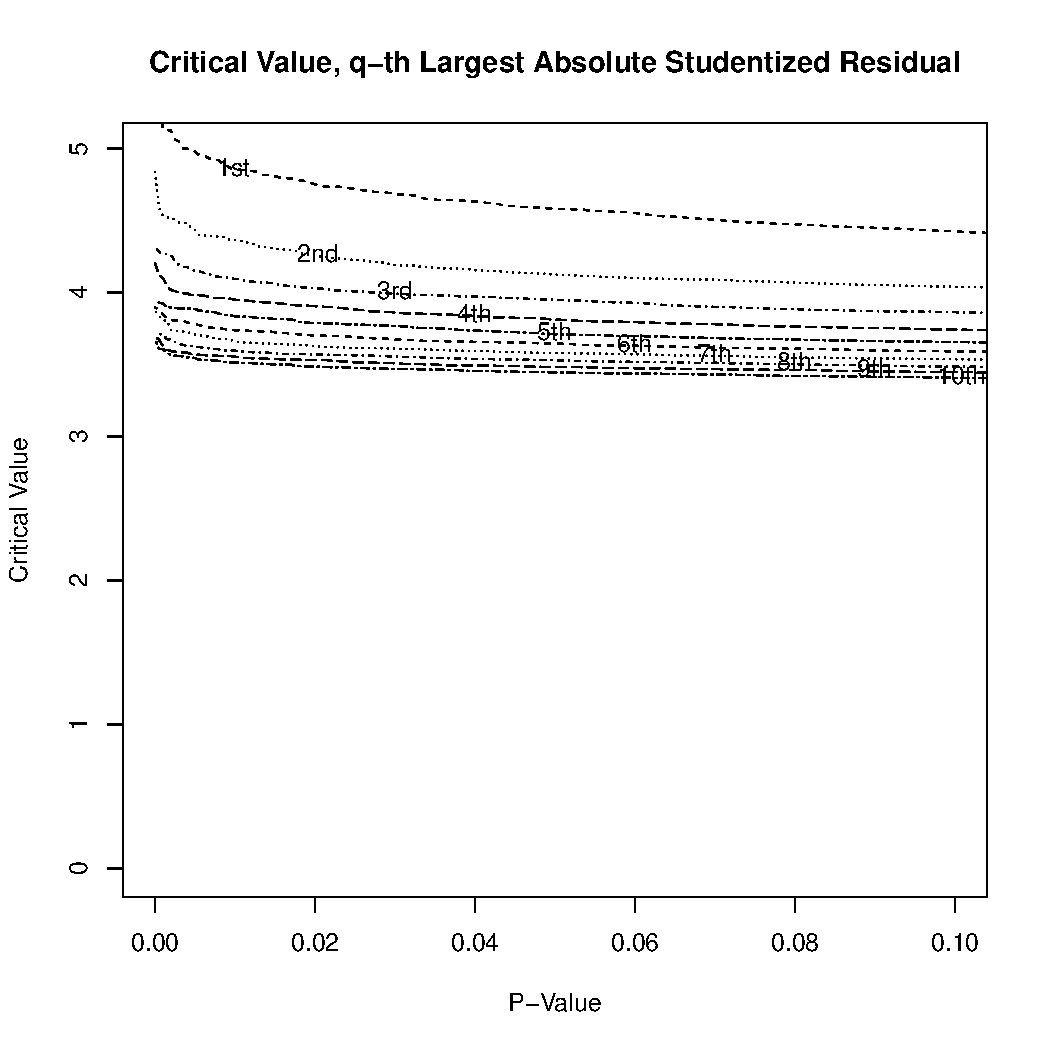
\includegraphics[width=12cm]{final/2bii_plot} 
                        \end{center}
                        Comparing the absolute value of $1$st-$10$th largest studentized residuals from the original model:\\ 
                        \lstinputlisting[firstline=44,lastline=45]{final/2_out.txt} 
                        To the respective critical values at p-values of $.01$, $.05$, and $.1$: \\
                        \lstinputlisting[firstline=47,lastline=50]{final/2_out.txt} 
                        We see that they all fall outside of the critical values for each confidence level, so we would reject them all as outliers for each confidence level. This fits with the simpler Bonferroni Critical value we used before; since it is conservative, and each of the studentized residuals falls above it, it stands to reason a sharper test would reject them to. \\
                        {\bf My R Code:}
                        \lstinputlisting[firstline=231,lastline=247,breaklines=true]{final.R} 

                    
                \end{itemize}
            \item[c)]
                From what we've seen, these few extreme points clearly don't fit the assumptions for the simple linear model on the variables we have, which in general seems appropriate for the vast majority of the data. In that sense they are certainly outliers to that model. However, they are not necessarily outliers due to mismeasurement or some other factor such that they should be thrown out as invalid or impossible to include in a linear model. For instance, it may be the case that they represent periods during which their was a mechanical breakdown of some sort. If this were true, we could include them in the model if we had information about mechanical failures at the power plant to include in the model. Then they might well fit the assumptions for a standard linear model. 
        \end{itemize}
    \item[3.]
        \begin{itemize}
            \item[a)]
                Of the shrinkage methods we have discussed, PLS and Lasso are particularly suitable for $n<p$, while PCR is still ok but not as good as the other two. PLS and Lasso are best because they attempt to pick a sparse representation of the predictor space which predicts the outcome well. PLS does this by selecting components of a orthonormal basis in order of their predictiveness, while LASSO, depending at which point it is cut off, adds the original predictors back in as they increase predictive power, keeping the coefficients for the rest at $0$. Both of these processes result in a smaller, predictive subspace, effectively reducing $p$. PCR also shrinks the predictor space, but since it selects the orthogonal components which represent the largest variation in the predictor space, rather than are the most predictive of the outcome, it will likely give a subspace of larger dimension. For instance, in an extreme case, if the largest $n$ primary components don't predict the outcome at all, PCR will fail. Ridge regression is the least suitable option, since it only rarely will out right eliminate a predictor, instead constraining the size of $\|\beta\|_2$ over all predictors.
            \item[b)]
                I fit a PCR model to the permuted training set, using ``pcr" in R, and then selected the number of components from the Scree plot and 10 fold cross validation. I chose 10 fold cross validation for a few reasons. First, with a relatively small number of observations in the test data set, using a smaller $k$ would result in a data set that is small enough to have meaningfully different error properties (since reducing a data set by a set portion increases the prediction error the most when the data set is small). Larger $k$ on the other hand would increasingly look like LOO cross validation. Besides, that though, the choice is somewhat arbitrary, so I went with common wisdom on the subject. The Scree plot and plotted cross validation scores are below: \\
                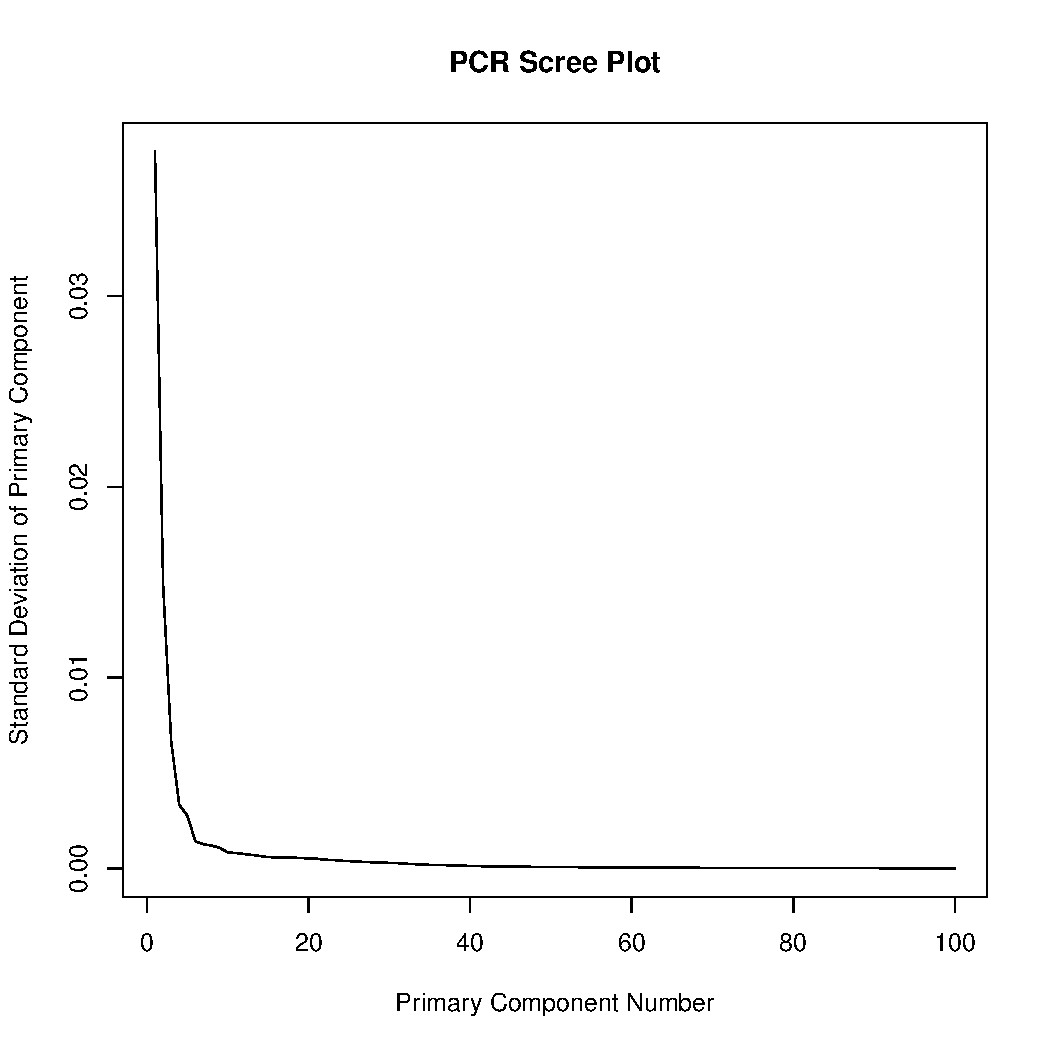
\includegraphics[width=9cm]{final/3b_pcr_scree} 
                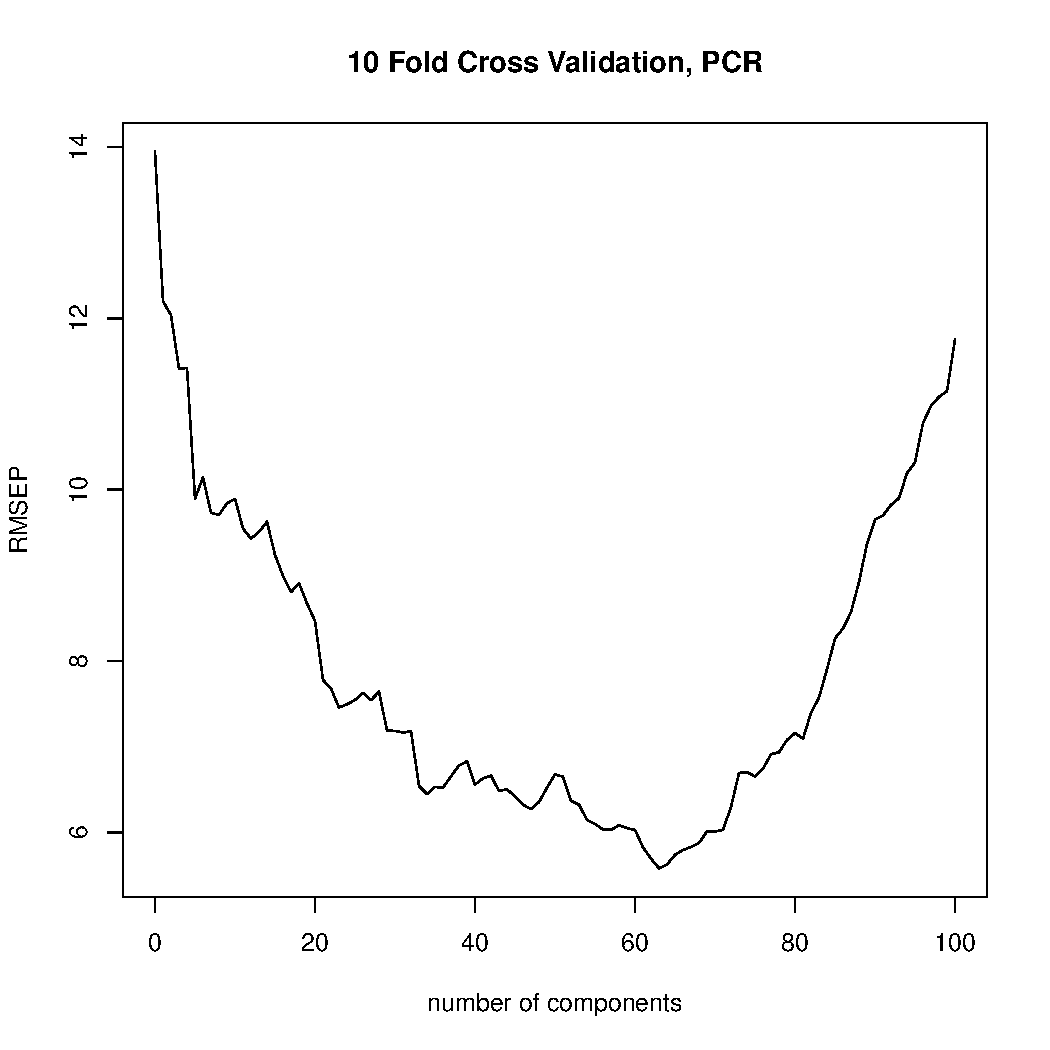
\includegraphics[width=9cm]{final/3b_pcr_cv} \\ 
                The Scree plot vaguely seemed to have an elbow at 10, where the marginal fall off of the standard deviations for each principal component slowed down, so I tried a model with 10 components. On the test set, the predictions from this model gave a RMSE of $8.69$. Going by $10$ fold cross validation, including $64$ components resulted in the lowest predicted RMSE of $5.58$. The actual RMSE of the test data set was $5.65$ for this model.
            \item[c)]
                I fit a PLS model, using ``plsr" in R. I plotted out the $10$ fold cross validation scores:
                \begin{center}
                    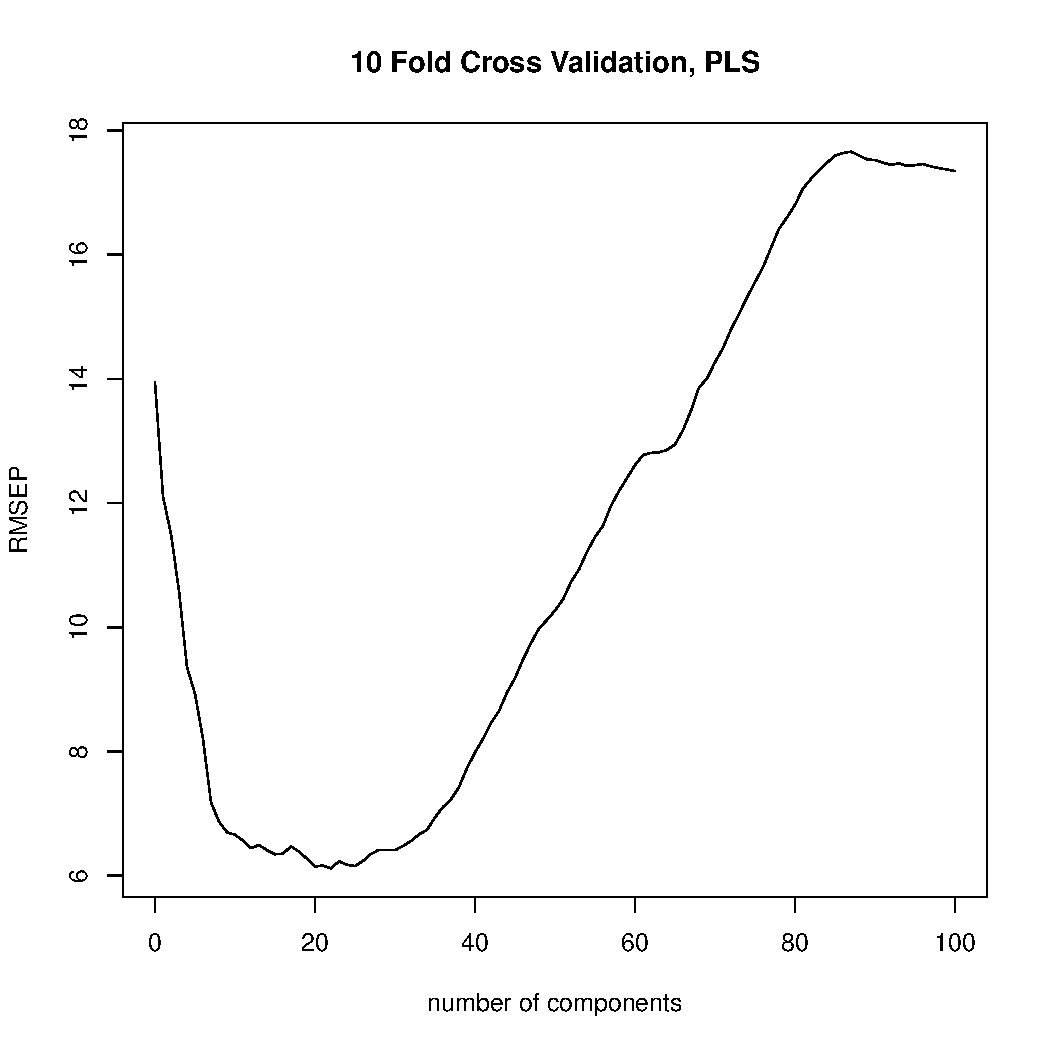
\includegraphics[width=9cm]{final/3c_pls_cv} 
                \end{center}
                The predicted RMSE was minimized by $23$ components, a much smaller number than with PCR, predicting a RMSE of $6.12$. In fact, it turned out the actual RMSE on the test data set was $5.15$.
            \item[d)]
                Fitting both of these models again, but this time fitting the number of components by LOO cross validation, we get these predictions for RMSE: \\
                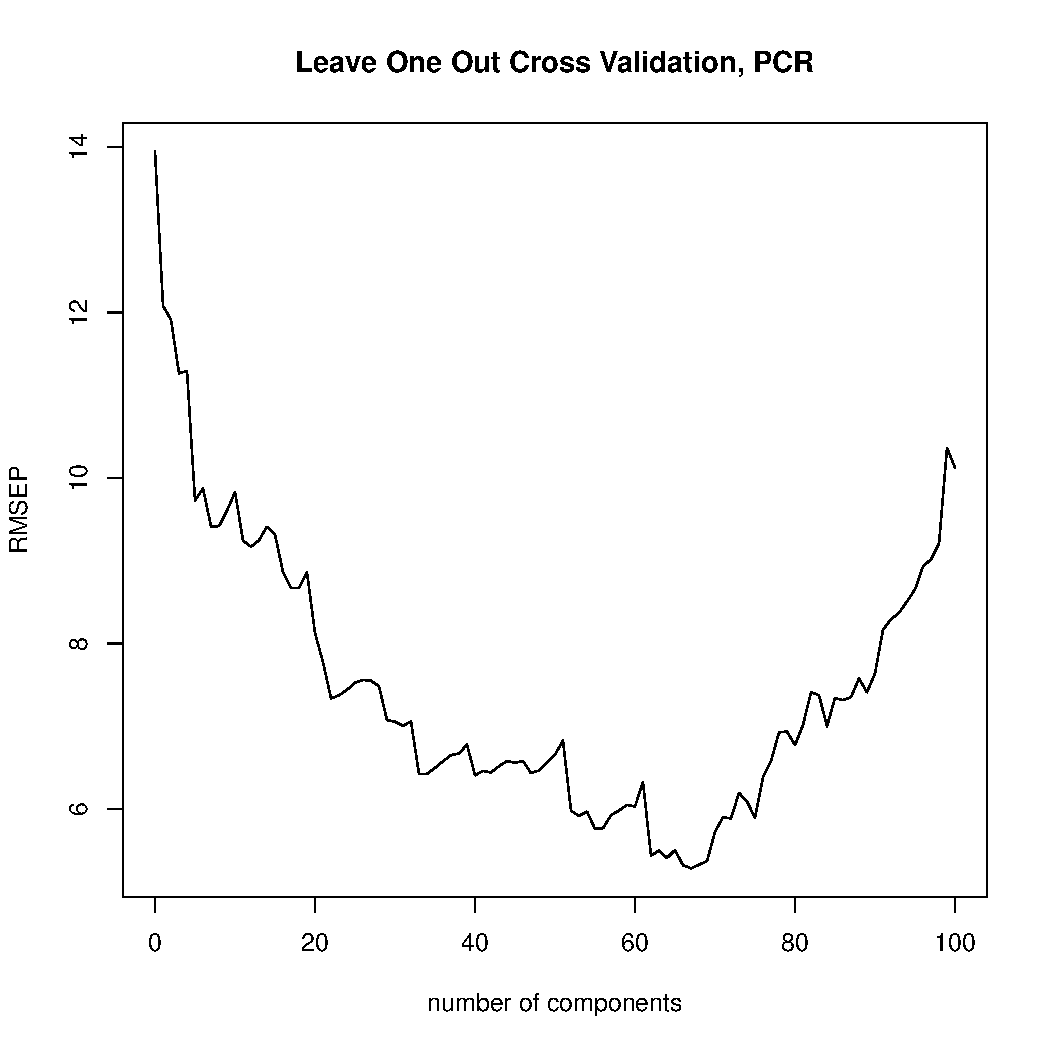
\includegraphics[width=9cm]{final/3d_pcr_loo} 
                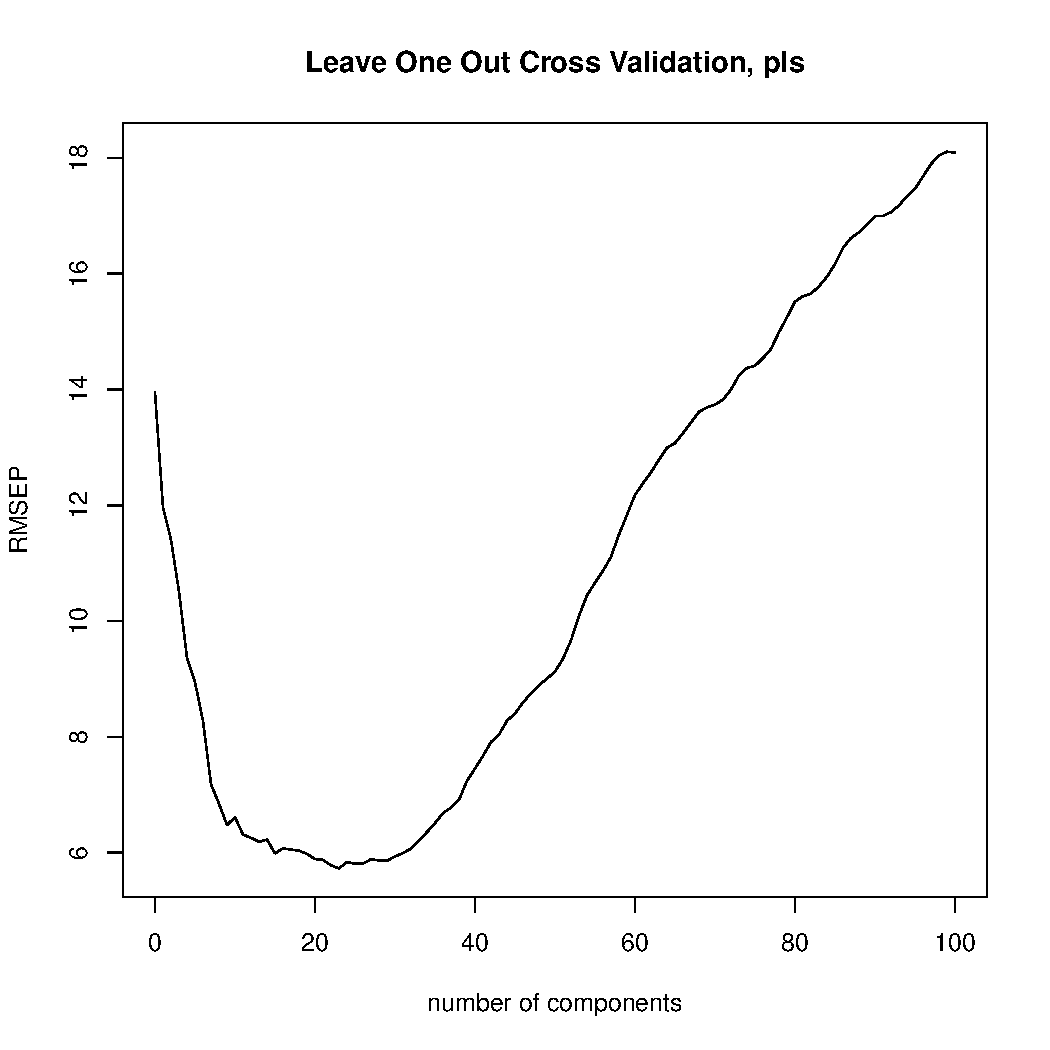
\includegraphics[width=9cm]{final/3d_pls_loo} \\ 
                As you can see, they are very similar, though not quite identical, to the results from $10$ fold cross validation. For PCR, the minimum is now found at $68$ components, with a predicted RMSE of $5.28$; this results in an actual RMSE on the test data set of $5.64$. For PLS, the minimum is at $24$ components, predicting a $RMSE$ of $5.57$ compared to an actual RMSE on the test set of $5.26$. \par
                Both methods result in pretty similar models with similar performance on the test data set; the PLS model chosen from LOO was a bit worse from the one chosen from $10$ fold, but the PCR model was a hair better. The differences are small enough to be regarded as mere noise though. The only really distinction between the methods is that LOO predicted the actual RMSE for PLS far better than $10$ fold, though the models end up being almost identical. This is about what I expected; the error in fitting a model fit on $n-1$ data points should be more similar to one fit on $n$ data points than one fit on $\frac{9n}{10}$ data points.
            \item[e)]
                I fit a LASSO model using the ``lars" command in R. In the same package, there is ``cv.lars", which calculates cross validation scores. It subsets the data into $K$ parts and fits a full LASSO model on each combination of $K-1$ of the $K$ subsets. Then, for a set of complexity parameters given by the user, calculates the RMSE of each model on the subset of the data it wasn't fit over. The average of the RMSE calculations from the $K$ models is then the predicted out of sample RMSE. I made use of this, using $10$ folds, to choose the complexity parameter.
 Below is the graph of the RMSE at different complexity parameters, and a small portion of the LASSO plot: \\   
                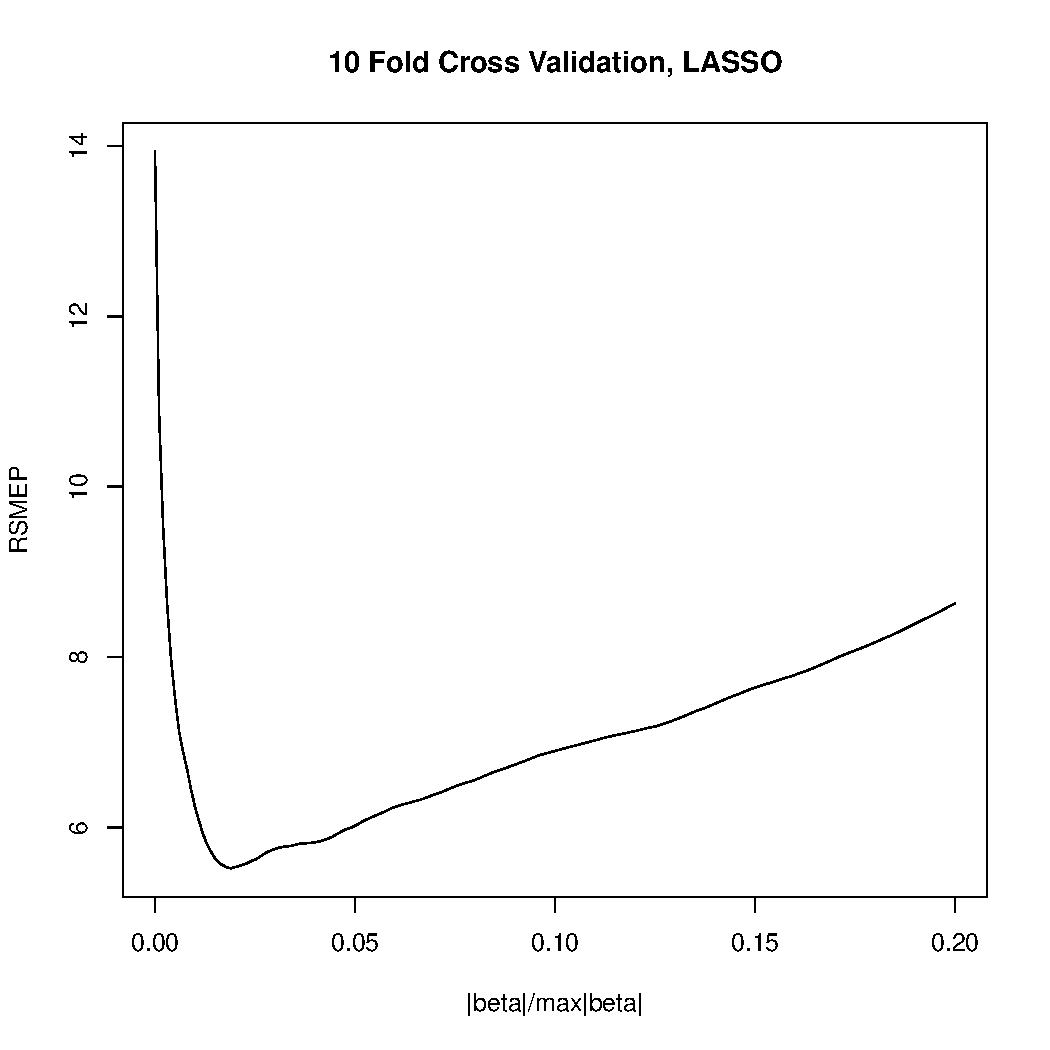
\includegraphics[width=9cm]{final/3e_cv_plot}
                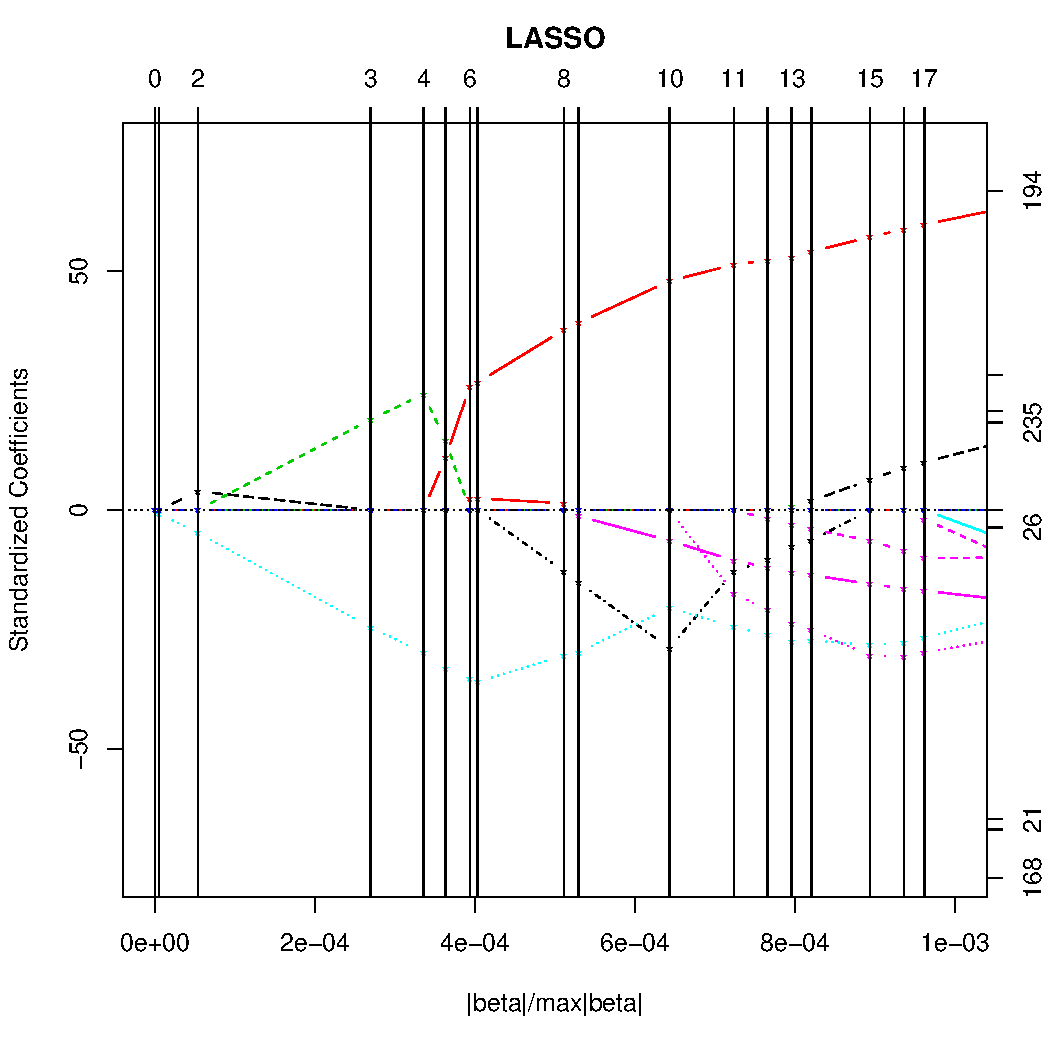
\includegraphics[width=9cm]{final/3e_lasso_plot} \\ 
                The best complexity parameter according to $10$ fold cross validation was \(.019=\frac{\|\beta\|_1}{\max\|\beta\|_1}\), with an estimated RMSE of $5.52$. This gave 38 variables with positive coefficients. On the test data set, this model's predictions had a RMSE of $5.33$. \par
                Of these three methods, I like PLS the best. It seems better than PCR, since it gives only the components that are actually predictive, so includes far fewer. LASSO results in more predictors, but uses the actual original variables, so it certainly has its value too; I find the pleasant mathematically properties of orthogonal predictors appealing though, even if they are harder to interpret. 
            \item[f)]
                The biggest advantage of K-fold CV is that, assuming there isn't a simple closed form for LOO CV as with linear smoothers, it is much quicker to run; the  model only has to be run $K$ times, instead of $n$ times, saving a lot of computation. It also has the advantage of less variance than LOO. Since each model for LOO is fit on a nearly identical data set, the prediction errors will be highly correlated. On the other hand, each of the models for $K$ fold are for more distinct, making the prediction errors less correlated, and the resulting mean less noisy. LOO CV will produce a less biased estimate of RMSE though; models fit on less data will tend to have somewhat higher error. Thus, identical models fit on $n$ and $n-1$ data points, as with LOO CV, will have a more similar error distribution than identical models fit on $n$ and $n\frac{k-1}{k}$ data points, as with $K$-fold CV (unless $k=n$).

        \end{itemize}
\end{itemize}

\end{document}
